%-------- Ignore -----------

%-----------------------------------------------------------------------------------------------------------%
\newpage

\part{پیشنیاز های ریاضی}
{
    \Large
    \begin{spacing}{1.4}
        \textbf{\vspace{3pt}}
        \begin{displayquote}
            راجر بیکن: زیرا چیزهای این جهان را نمی توان بدون دانش ریاضیات شناخت.
            \begin{flushleft}
                \lr{Opus Majus part 4 Distinctia Prima cap 1, 1267.}
            \end{flushleft}
        \end{displayquote}
        \textbf{\vspace{3pt}}

        بازی های ویدیویی سعی در شبیه سازی دنیای مجازی دارند.
        با این حال، کامپیوترها، به دلیل ماهیت خود، اعداد را محاسبه می کنند. بنابراین مشکل چگونگی انتقال جهان به کامپیوتر مطرح می شود.
        پاسخ این مشکل اینگونه است که جهان‌های ما و فعل و انفعالات موجود در آن را کاملاً ریاضی توصیف کنیم.
        در نتیجه، ریاضیات نقش اساسی در توسعه بازی های ویدیویی ایفا می کند.

        در این بخش، ابزارهای ریاضی که در این کتاب مورد استفاده قرار گرفته اند، معرفی می کنیم. تأکید ما بر بردارها، سیستم های مختصات، ماتریس ها و تبدیل ها است، زیرا این ابزارها تقریباً در همه ی برنامه های نمونه این کتاب استفاده شده اند.
        علاوه بر توضیحات ریاضی، بررسی و نمایش کلاس ها و توابع مربوطه از کتابخانه ریاضی \lr{DirectX} را نیز ارائه میکنیم.

        توجه داشته باشید که موضوعاتی که در اینجا مورد بررسی قرار می‌گیرند، تنها مواردی هستند که برای درک ادامه ی این کتاب ضروری اند.
        این کتاب به هیچ وجه راه حل جامعی برای ریاضیات بازی های ویدیویی نیست.

        \begin{point}{pnt:1}
            \Large
            برای خوانندگانی که مایل به ارجاع کامل تر به ریاضیات بازی های ویدیویی هستند، کتاب های زیر را توصیه می کنیم.
            \lr{
                \begin{enumerate}[label=\textbf{\arabic*}.]
                    \item {Essential Mathematics for Games and Interactive Applications: A Programmer's Guide (Verth04)}
                    \item {Mathematics for 3D Game Programming and Computer Graphics (Lengyel02)}
                \end{enumerate}
            }
            \textbf{\vspace{-20pt}}
        \end{point}

        \textbf{فصل 1، جبر برداری:} بردارها اساسی ترین اشیاء ریاضی مورد استفاده در بازی های کامپیوتری هستند.
        ما از بردارها برای نشان دادن موقعیت ها، جابجایی ها، جهت ها، سرعت ها و نیروها استفاده می کنیم.
        در این فصل، بردارها و عملیات مورد استفاده برای کار با آنها را مطالعه می کنیم.

        \textbf{فصل 2، جبر ماتریسی:} ماتریس ها روشی کارآمد و فشرده برای نمایش تبدیل ها ارائه می دهند.
        در این فصل با ماتریس ها و عملیات تعریف شده بر روی آنها آشنا می شویم.

        \textbf{فصل 3، تبدیل:} این فصل سه تبدیل هندسی اساسی را بررسی می کند: مقیاس بندی، چرخش و انتقال.
        ما از این تبدیل ها برای کار با اشیاء سه بعدی در فضا استفاده می کنیم.
        علاوه بر این، تغییر تبدیل مختصات را توضیح می دهیم، که برای تبدیل مختصات هندسی از یک سیستم مختصات به سیستم دیگر استفاده می شود.
    \end{spacing}
}

\setcounter{chapter}{1}

\textbf{\vspace{80pt}}


\chapter{\textbf{1 جبر برداری}}
\textbf{\vspace{70pt}}
{
    \Large
    \begin{spacing}{1.5}
        بردارها نقش مهمی در گرافیک کامپیوتری، تشخیص برخورد و شبیه سازی فیزیکی ایفا می کنند که همگی اجزای رایج در بازی های ویدئویی مدرن هستند.
        رویکرد ما در اینجا غیر تخصصی و عملی است به همین دلیل پیشنهاد ما کتاب \lr{Verth04} (نکته \ref{pnt:1}) است که کتابی اختصاصی برای ریاضیات بازی های سه بعدی/گرافیک است.
        ما بر اهمیت بردارها بسیار تأکید داریم زیرا در بیشتر برنامه های آزمایشی این کتاب استفاده شده اند.
        \\

        \textbf{\LARGE \hspace{-40pt}اهداف:}
        \begin{enumerate}[label=\textbf{\arabic*}.]
            \item {یادگیری نحوه نمایش بردارها به صورت هندسی و عددی}
            \item {یادگیری عملیات تعریف شده بر روی بردارها و کاربردهای هندسی آنها}
            \item {آشنایی با توابع برداری و کلاس های کتابخانه \lr{DirectXMath}}
        \end{enumerate}
    \end{spacing}
}
%-----------------------------------------------------------------------------------------------------------%
\newpage

\setcounter{figure}{0}
\renewcommand{\thefigure}{\arabic{figure}.\arabic{chapter}}

\section{\textbf{بردار ها}}
{
    \Large
    \begin{spacing}{1.4}
        بردار به کمیتی اشاره دارد که هم اندازه و هم جهت دارد.
        به کمیت هایی که اندازه و جهت دارند، کمیت های برداری گویند.
        نمونه‌هایی از کمیت‌های برداری عبارتند از نیروها (نیرو در جهت خاصی با قدرت/اندازه معین اعمال می‌شود)، جابه‌جایی (جهت برآیند و فاصله حرکت ذره)، و سرعت‌ها (سرعت و جهت).
        بنابراین، بردارها برای نمایش نیروها، جابجایی ها و سرعت ها استفاده می شوند.
        به علاوه، ما از بردارها برای تعیین جهات خالص استفاده می کنیم،
        مانند جهتی که بازیکن در یک بازی سه بعدی به آن نگاه میکند،
        جهتی که یک چند ضلعی رو به آن قرار دارد، جهتی که پرتوی نور در آن حرکت می کند،
        یا جهتی که در آن یک پرتو نور از یک سطح منعکس می شود.

        اولین مرحله در توصیف ریاضی بردار ، توصیف هندسی آن است: ما به صورت گرافیکی یک بردار را با یک پاره خط جهت دار مشخص می کنیم (شکل \ref{fig:4.Session.1.1.1})، که در آن طول نشان دهنده بزرگی بردار و سر کمان نشان دهنده جهت بردار است.
        به این نکته باید توجه کنید که مکانی که در آن یک بردار رسم می‌کنیم بی‌اهمیت است، زیرا تغییر مکان، بزرگی یا جهت را تغییر نمی‌دهد (دو ویژگی ای که بردار دارد).
        بنابراین می گوییم دو بردار برابر هستند اگر و تنها اگر طول یکسانی داشته و در یک جهت باشند.
        بنابراین، بردارهای \textbf{u} و \textbf{v} ترسیم شده در قسمت آ شکل \ref{fig:4.Session.1.1.1} در واقع برابر اند زیرا طول و جهت یکسانی دارند.
        در واقع، چون مکان برای بردارها اهمیتی ندارد، ما می‌توانیم یک بردار را بدون تغییر ماهیت آن ، انتقال دهیم (زیرا انتقال نه طول و نه جهت را تغییر می‌دهد).
        توجه داشته باشید که ما می‌توانیم \textbf{u} را طوری انتقال دهیم که کاملاً بر \textbf{v} همپوشانی داشته باشد (و بالعکس) و در نتیجه آنها را غیرقابل تشخیص کنیم. این نیز دلیلی برای برابری آنهاست.

        \begin{figure}[H]
            \centering
            \setlength{\belowcaptionskip}{-10pt}
            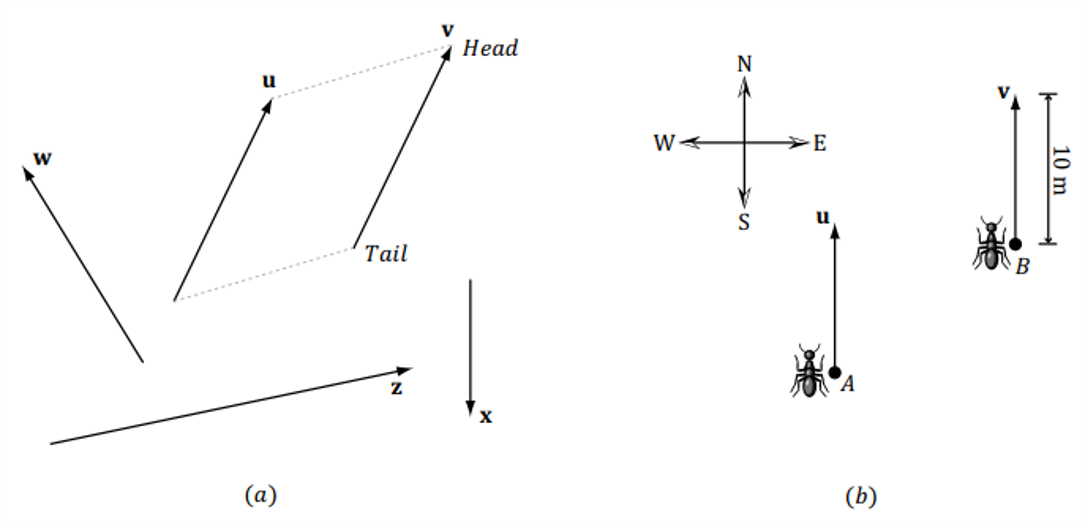
\includegraphics[width=0.85\textwidth]{Images/4/1/4.Session.1.1.1}
            \caption{(الف) بردار هایی که روی صفحه ی دوبعدی کشیده شده اند.
                (ب) بردار هایی که مورچه ها را برای حرکت 10 متر در جهت شمال راهنمایی میکنند.}
            \label{fig:4.Session.1.1.1}
        \end{figure}

        به عنوان یک مثال فیزیکی، بردارهای \textbf{u} و \textbf{v} در قسمت ب شکل \ref{fig:4.Session.1.1.1} هر دو به مورچه ها میگویند در دو نقطه مختلف \lr{A} و \lr{B} ده متر به سمت شمال حرکت کنند.
        دوباره \lr{\textbf{u} = \textbf{v}} را داریم.
        بردارها خود مستقل از موقعیت هستند و
        آنها به سادگی به مورچه ها آموزش می دهند که چگونه از جایی که هستند، ده متر (طول) به سمت شمال (جهت) حرکت کنند.

    \end{spacing}
}

\subsection{\textbf{عملیات بردار پایه}}
{
    \Large
    \begin{spacing}{1.5}
        اکنون با استفاده از نمایش مختصاتی، تساوی، جمع، ضرب اسکالر و تفریق را بر روی بردارها تعریف می کنیم.
        برای این چهار تعریف، فرض میکنیم $\textbf{u}=(u_{x},u_{y},u_{z})$ و  $\textbf{v}=(v_{x},v_{y},v_{z})$.

        \begin{enumerate}[label=\textbf{\arabic*}.]
            \item {دو بردار مساوی هستند اگر و تنها اگر اجزای متناظر آنها با هم برابر باشند.
            یعنی $\textbf{u}=\textbf{v}$ اگر و تنها اگر $u_{x}=v_{x}$ ، $u_{y}=v_{y}$ و $u_{z}=v_{z}$}
            \item {بردارها را به صورت جزء اضافه می کنیم: $\textbf{u}+\textbf{v}=(u_{x}+v_{x},u_{y}+v_{y},u_{z}+v_{z})$.
            توجه داشته باشید که فقط اضافه کردن بردارهایی با همان بعد ، منطقی ست.}
            \item {می توانیم یک اسکالر (یعنی یک عدد حقیقی) و یک بردار را ضرب کنیم و نتیجه یک بردار خواهد بود.
            فرض کنید k یک اسکالر باشد، پس $k\textbf{u}=(ku_{x},ku_{y},ku_{z})$. به این ضرب اسکالر می گویند.}
            \item {ما تفریق را بر حسب جمع بردار و ضرب اسکالر انجام می دهیم.
            یعنی\\$\textbf{u}\textbf{-v}=\textbf{u}+(-1\cdot\textbf{v})=\textbf{u}+(\textbf{-v})=(u_{x}-v_{x},u_{y}-v_{y},u_{z}-v_{z})$}
        \end{enumerate}

        \textbf{\vspace{-10pt}}
        \begin{example}{exp:1.1}
            \Large
            فرض کنید $\textbf{u}=(1,2,3), \textbf{v}=(1,2,3), \textbf{w}=(3,0,-2), k=2$
            \lr{
                \begin{enumerate}[label=\textbf{\arabic*}.]
                    \item {$\textbf{u}+\textbf{w}=(1,2,3)+(3,0,-2)=(4,2,1)$}
                    \item {$\textbf{u}=\textbf{v}$}
                    \item {$\textbf{u}-\textbf{v}=\textbf{u}+(\textbf{-v})=(1,2,3)+(-1,-2,-3)=(0,0,0)=\textbf{0}$}
                    \item {$k\textbf{w}=2(3,0,-2)=(6,0,-4)$}
                \end{enumerate}
            }
            تفاوتی که در مورد سوم هست ، یک بردار خاص به نام بردار صفر را نشان می دهد که همه اجزای آن صفر است و با \lr{\textbf{0}} نشان داده می شود.
        \end{example}

        \textbf{\vspace{-20pt}}
        \begin{example}{exp:1.2}
            \Large
            ما این مثال را با بردارهای دوبعدی برای ساده‌تر کردن کار توضیح می‌دهیم. ایده ها مانند فضای سه بعدی هستند، فقط با یک جزء کمتر ، به صورت دو بعدی کار می کنیم.\\
            \begin{enumerate}[label=\textbf{\arabic*}.]
                \item {فرض کنید $\textbf{v}=(2,1)$، $\textbf{v}$ و $-\frac{\displaystyle 1}{\displaystyle 2}\textbf{v}$ چگونه از نظر هندسی با هم مقایسه می شوند؟
                توجه داریم که $-\frac{\displaystyle 1}{\displaystyle 2}\textbf{v}=(-1,-\frac{\displaystyle 1}{\displaystyle 2})$.
                با ترسیم نمودار $\textbf{v}$ و $-\frac{\displaystyle 1}{\displaystyle 2}\textbf{v}$ (قسمت آ شکل \ref{fig:4.Session.1.1.6})،
                متوجه می‌شویم که $-\frac{\displaystyle 1}{\displaystyle 2}\textbf{v}$ در جهت مخالف $\textbf{v}$ است و طول آن $\frac{\displaystyle 1}{\displaystyle 2}\textbf{v}$ است.
                بنابراین، از نظر هندسی، منفی کردن یک بردار را می‌توان به صورت "برگرداندن" جهت آن،
                و ضرب اسکالر را می توان به عنوان مقیاس بندی طول یک بردار در نظر گرفت.}\\

                \item {فرض کنید $\textbf{u}=(2,\frac{\displaystyle 1}{\displaystyle 2})$ و $\textbf{v}=(1,2)$. پس $\textbf{u}+\textbf{v}=(3,\frac{\displaystyle 5}{\displaystyle 2})$ .
                قسمت ب شکل \ref{fig:4.Session.1.1.6} نشان می‌دهد که جمع بردار از نظر هندسی به چه معناست:
                ما $\textbf{u}$ را به‌طور موازی انتقال میدهیم تا دم آن با سر $\textbf{v}$ منطبق شود.
                پس بردار مجموع ، برداری است که از دم $\textbf{v}$ شروع شده و با سر $\textbf{u}$ منتقل شده ختم می‌شود.
                    (اگر $\textbf{u}$ را ثابت نگه داریم و $\textbf{v}$ را طوری انتقال دهیم که دم آن با سر $\textbf{u}$ منطبق شود، همین نتیجه را می گیریم.
                    در این حالت، $\textbf{u}+\textbf{v}$ برداری خواهد بود که از دم $\textbf{u}$ شروع شده و با سر $\textbf{v}$ منتقل شده ختم میشود.)
                    توجه داشته باشید که قوانین جمع بردار در زمانی که نیروها را با هم جمع می کنیم تا نیروی برآیند را به وجود بیاوریم، با انتظار ما مطابقت دارد:
                    اگر دو نیرو (بردار) را در یک راستا اضافه کنیم، نیروی برآیند قوی تری (بردار طولانی تر) در آن جهت دریافت می کنیم.
                    اگر دو نیرو (بردار) مخالف یکدیگر را بهم اضافه کنیم، نیروی برآیند ضعیف تری (بردار کوتاه تر) به دست می آید.
                    شکل \ref{fig:4.Session.1.1.7} این ایده ها را نشان می دهد.}\\

                \item {فرض کنید $\textbf{u}=(2,\frac{\displaystyle 1}{\displaystyle 2})$ و $\textbf{v}=(1,2)$. پس $\textbf{v}-\textbf{u}=(-1,\frac{\displaystyle 3}{\displaystyle 2})$.
                قسمت پ شکل \ref{fig:4.Session.1.1.6} نشان می دهد که تفریق برداری از نظر هندسی به چه معناست.
                    $\textbf{v}-\textbf{u}$ به ما یک بردار با از سر $\textbf{u}$ تا سر $\textbf{v}$ می دهد.
                    اگر در عوض $\textbf{u}$ و $\textbf{v}$ را به عنوان نقاط تفسیر کنیم، آنگاه $\textbf{v}-\textbf{u}$ برداری را با هدف از نقطه $\textbf{u}$ تا نقطه $\textbf{v}$ به ما می دهد.
                    این تفسیر مهم است زیرا ما اغلب می خواهیم که بردار از یک نقطه به نقطه دیگر برود.
                    همچنین طول $\textbf{v}-\textbf{u}$ فاصله $\textbf{u}$ تا $\textbf{v}$ است، وقتی که $\textbf{u}$ و $\textbf{v}$ را به عنوان نقطه در نظر بگیریم.}
            \end{enumerate}

            \begin{figure}[H]
                \centering
                \setlength{\belowcaptionskip}{-10pt}
                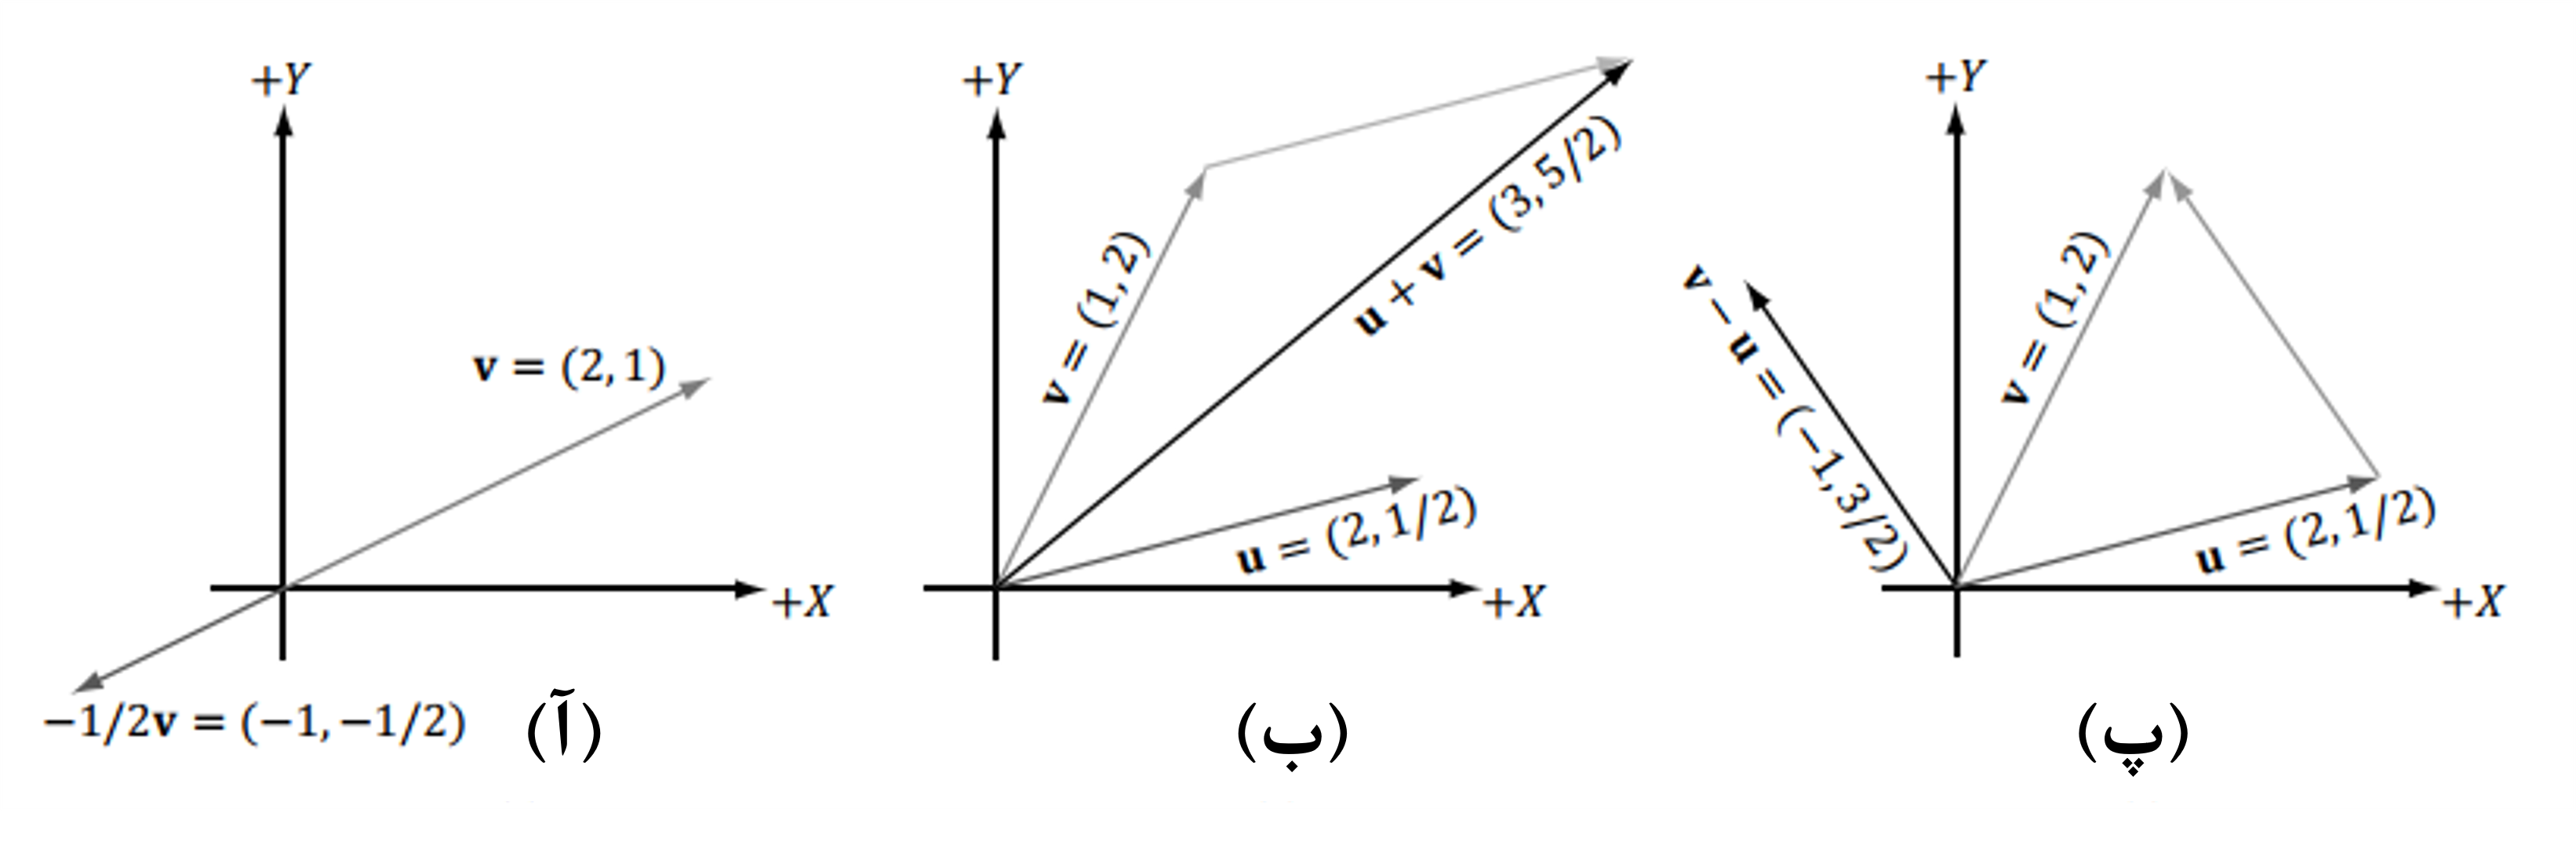
\includegraphics[width=\textwidth]{Images/4/1/4.Session.1.1.6}
                \caption{(آ) تفسیر هندسی ضرب اسکالر. (ب) تفسیر هندسی جمع بردار. ج) تفسیر هندسی تفریق بردار.}
                \label{fig:4.Session.1.1.6}
            \end{figure}

            \begin{figure}[H]
                \centering
                \setlength{\belowcaptionskip}{-10pt}
                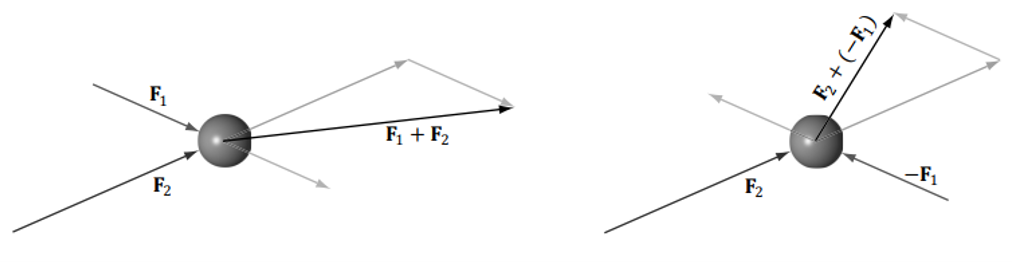
\includegraphics[width=\textwidth]{Images/4/1/4.Session.1.1.7}
                \caption{نیروهای اعمال شده به یک توپ. نیروها با استفاده از جمع بردار ترکیب می شوند تا نیروی برآیند به دست آید. \textbf{\vspace{10pt}}}
                \label{fig:4.Session.1.1.7}
            \end{figure}
        \end{example}
    \end{spacing}
}

\section{\textbf{بردارهای طول و واحد}}
{
    \Large
    \begin{spacing}{1.5}
        از نظر هندسی اندازه ی یک بردار، طول پاره خطی جهت دار است.
        اندازه ی یک بردار را با خط های عمودی دوتایی نشان می دهیم
        (به عنوان مثال، $\norm{u}$ اندازه ی $\textbf{u}$ را نشان می دهد).
        حالا با توجه به بردار $\textbf{u}=(x,y,z)$، می‌خواهیم بزرگی آن را به صورت جبری محاسبه کنیم.
        اندازه ی یک بردار سه بعدی را می توان با دو بار اعمال قضیه فیثاغورث محاسبه کرد.
        شکل \ref{fig:4.Session.1.1.8} را ببینید. ابتدا، ما به مثلث در صفحه $xz$ با اضلاع $x$، $z$ و وتر $a$ نگاه می کنیم.

        \begin{figure}[H]
            \centering
            \setlength{\belowcaptionskip}{-10pt}
            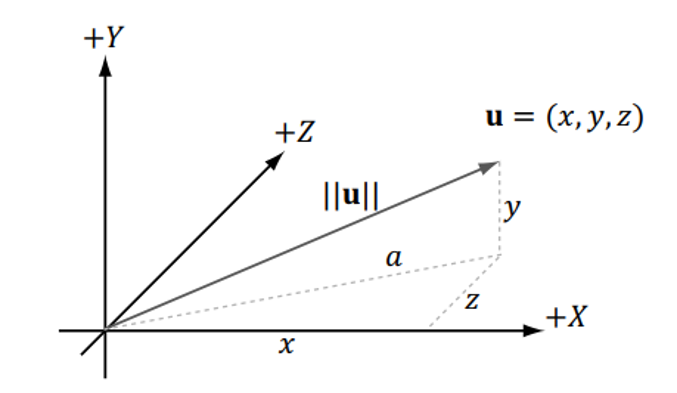
\includegraphics[width=0.5\textwidth]{Images/4/1/4.Session.1.1.8}
            \caption{طول سه بعدی یک بردار را می توان با دو بار اعمال قضیه فیثاغورث محاسبه کرد.}
            \label{fig:4.Session.1.1.8}
        \end{figure}

        از قضیه فیثاغورث، $a=\sqrt{\displaystyle x^2+z^2}$ داریم.
        حالا به مثلث با ضلع های \lr{a}، \lr{y} و وتر $\norm{u}$ نگاه کنید از قضیه فیثاغورث دوباره به فرمول اندازه ی زیر می رسیم:

        \begin{eqtn}{eqtn:1}
            \centering
            $\norm{\textbf{u}}=\sqrt{\displaystyle y^2+a^2}=\sqrt{\displaystyle y^2+(\sqrt{\displaystyle x^2+z^2})^2}=\sqrt{\displaystyle x^2+y^2+z^2}$
        \end{eqtn}

        برای برخی از استفاده ها، ما به طول یک بردار اهمیتی نمی دهیم زیرا می خواهیم از بردار برای نمایش یک جهت خالص استفاده کنیم.
        می خواهیم طول چنین بردارهایی با فقط یک جهت دقیقاً 1 باشد.
        وقتی طول واحد برداری را می سازیم، می گوییم که بردار را نرمال کرده ایم.
        می توانیم یک بردار را با تقسیم هر یک از اجزای بر بزرگی آن ، نرمال کنیم:

        \begin{eqtn}{eqtn:2}
            \centering
            $\hat{\textbf{u}}=\frac{\displaystyle\textbf{u}}{\displaystyle\norm{\textbf{u}}}=\left(\frac{\displaystyle x}{\displaystyle\norm{\textbf{u}}},
            \frac{\displaystyle y}{\displaystyle\norm{\textbf{u}}}, \frac{\displaystyle z}{\displaystyle\norm{\textbf{u}}}\right)$
        \end{eqtn}

        برای تأیید صحت این فرمول، می توانیم طول $\hat{\textbf{u}}$ را محاسبه کنیم:

        \begin{center}
            $\norm{\hat{\textbf{u}}}=\sqrt{\displaystyle \left(\frac{\displaystyle x}{\displaystyle\norm{\textbf{u}}}\right)^2,
                \left(\frac{\displaystyle y}{\displaystyle\norm{\textbf{u}}}\right)^2,
                \left(\frac{\displaystyle z}{\displaystyle\norm{\textbf{u}}}\right)^2}=\frac{\displaystyle x^2+y^2+z^2}{\displaystyle\sqrt{\displaystyle \norm{\textbf{u}}^2}}
            =\frac{\displaystyle\norm{\textbf{u}}}{\displaystyle\norm{\textbf{u}}}=1$
        \end{center}

        پس $\hat{\textbf{u}}$ در واقع یک بردار واحد است.

        \begin{example}{exp:1.3}
            بردار $\textbf{v}=(-1,3,4)$ را نرمال کنید. داریم $\norm{\textbf{v}}=\sqrt{\displaystyle (-1)^2+3^2+4^2}=\sqrt{\displaystyle 26}$. پس:

            \begin{center}
                $\hat{\textbf{v}}=\frac{\displaystyle\textbf{v}}{\displaystyle\norm{\textbf{v}}}=\left(-\frac{\displaystyle 1}{\displaystyle\sqrt{\displaystyle 26}},
                \frac{\displaystyle 3}{\displaystyle\sqrt{\displaystyle 26}}, \frac{\displaystyle 4}{\displaystyle\sqrt{\displaystyle 26}}\right)$
            \end{center}

            برای تأیید اینکه $\hat{\textbf{v}}$ واقعاً یک بردار واحد است، طول آن را محاسبه می کنیم:

            \begin{center}
                $\norm{\hat{\textbf{v}}}=\sqrt{\displaystyle \left(-\frac{\displaystyle 1}{\displaystyle\sqrt{\displaystyle 26}}\right)^2,
                    \left(\frac{\displaystyle 3}{\displaystyle\sqrt{\displaystyle 26}}\right)^2, \left(\frac{\displaystyle 4}{\displaystyle\sqrt{\displaystyle 26}}\right)^2}=
                \sqrt{\displaystyle\frac{\displaystyle 1}{\displaystyle 26}+\frac{\displaystyle 9}{\displaystyle 26}+\frac{\displaystyle 16}{\displaystyle 26}}=\sqrt{\displaystyle 1}=1$
            \end{center}
        \end{example}
    \end{spacing}
}

%-------- Ignore -----------


%-----------------------------------------------------------------------------------------------------------%
\newpage

\setcounter{chapter}{2}
\setcounter{example}{0}
\setcounter{section}{0}

\textbf{\vspace{80pt}}


\chapter{\textbf{2 جبر ماتریسی}}
\textbf{\vspace{70pt}}
{
    \Large
    \begin{spacing}{1.5}
        در گرافیک کامپیوتری سه بعدی، ما از ماتریس ها برای توصیف فشرده تبدیل های هندسی مانند مقیاس بندی، چرخش و انتقال و همچنین برای تغییر مختصات یک نقطه یا بردار از یک سیستم مختصات به سیستم مختصات دیگر استفاده می کنیم.
        این فصل به بررسی ریاضیات ماتریس ها می پردازد.
        \\

        \textbf{\LARGE \hspace{-40pt}اهداف:}
        \begin{enumerate}[label=\textbf{\arabic*}.]
            \item {به دست آوردن درک درستی از ماتریس ها و عملیات تعریف شده بر روی آنها.}
            \item {یادگیری اینکه چگونه ضرب بردار-ماتریس را می توان به عنوان یک ترکیب خطی مشاهده کرد.}
            \item {یادگیری اینکه ماتریس همانی چیست و جابجایی، دترمینان و معکوس یک ماتریس چیست.}
            \item {برای آشنایی با زیرمجموعه کلاس ها و توابع ارائه شده توسط کتابخانه ریاضی \lr{DirectX} که برای ریاضیات ماتریسی استفاده می شود.}
        \end{enumerate}
    \end{spacing}
}
%-----------------------------------------------------------------------------------------------------------%
\newpage

\setcounter{figure}{0}
\renewcommand{\thefigure}{\arabic{figure}.\arabic{chapter}}


\section{\textbf{تعریف}}
\label{sec:2.1}
{
    \Large
    \begin{spacing}{1.5}
        یک ماتریس $m\times n$ ، $\textbf{M}$ آرایه مستطیلی از اعداد حقیقی با $m$ ردیف و $n$ ستون است.
        حاصل ضرب تعداد سطرها و ستون ها ابعاد ماتریس را نشان می دهد.
        اعداد موجود در یک ماتریس را عناصر ، ورودی یا درایه می نامند.
        ما یک عنصر ماتریسی را با مشخص کردن سطر و ستون عنصر با استفاده از نماد دوگانه $\textbf{M}_{ij}$ شناسایی می‌کنیم،
        جایی که زیرنویس اول ردیف را مشخص می‌کند و زیرنویس دوم ستون را مشخص می‌کند.

        \begin{example}{exp:2.1}
            \Large
            ماتریس های زیر را در نظر بگیرید:\\
            $\textbf{A}=\begin{bmatrix}
                            3.5 & 0  & 0                      & 0 \\
                            0   & 1  & 0                      & 0 \\
                            0   & 0  & 0.5                    & 0 \\
                            2   & -5 & \sqrt{\displaystyle 2} & 1
            \end{bmatrix}, \textbf{B}=\begin{bmatrix}
                                          B_{11} & B_{12} \\
                                          B_{21} & B_{22} \\
                                          B_{31} & B_{32}
            \end{bmatrix}, \textbf{u}=\begin{bmatrix}
                                          u_{1} & u_{2} & u_{3}
            \end{bmatrix}, \textbf{v}=\begin{bmatrix}
                                          1                      \\
                                          2                      \\
                                          \sqrt{\displaystyle 3} \\
                                          \pi
            \end{bmatrix}$
            \\
            \begin{enumerate}[label=\textbf{\arabic*}.]
                \item {ماتریس $\textbf{A}$ یک ماتریس $4\times 4$ است؛
                ماتریس $\textbf{B}$ یک ماتریس $3\times 2$ است؛
                ماتریس $\textbf{u}$ یک ماتریس $1\times 3$ است؛
                و ماتریس $\textbf{v}$ یک ماتریس $4\times 1$ است.}
                \item {عنصر را در ردیف چهارم و ستون دوم ماتریس $\textbf{A}$ با $A_{42}=-5$ شناسایی می کنیم. عنصر را در ردیف دوم و ستون اول ماتریس $\textbf{B}$ با $B_{21}$ شناسایی می کنیم.}
                \item {ماتریس‌های $\textbf{u}$ و $\textbf{v}$ ماتریس‌های خاصی هستند به این معنا که به ترتیب حاوی یک سطر یا ستون هستند.
                ما گاهی اوقات این نوع ماتریس ها را بردار ردیف یا بردار ستون می نامیم زیرا برای نمایش یک بردار به شکل ماتریس استفاده می شود
                    (به عنوان مثال، می توانیم آزادانه نمادهای برداری $(x, y, z)$ و $[x, y, z]$ را مبادله کنیم).
                    توجه داشته باشید که برای بردارهای ردیف و ستون، استفاده از یک زیرنویس دوگانه برای نشان دادن عناصر ماتریس غیر ضروری است (ما فقط به یک زیرنویس نیاز داریم.)}
            \end{enumerate}
            گاهی اوقات ما ردیف های یک ماتریس را به عنوان بردار در نظر میگیریم. برای مثال، ممکن است بنویسیم:

            $\begin{bmatrix}
                 A_{11} & A_{12} & A_{13} \\
                 A_{21} & A_{22} & A_{23} \\
                 A_{31} & A_{32} & A_{33}
            \end{bmatrix}=\begin{bmatrix}
                              \leftarrow & A_{1,*} & \rightarrow \\
                              \leftarrow & A_{2,*} & \rightarrow \\
                              \leftarrow & A_{3,*} & \rightarrow
            \end{bmatrix}$

            که $\textbf{A}_{1,*}=[A_{11},A_{12},A_{13}]$ ، $\textbf{A}_{2,*}=[A_{21},A_{22},A_{23}]$ و $\textbf{A}_{3,*}=[A_{31},A_{32},A_{33}]$ هستند.
            در این نماد، اندیس اول سطر را مشخص می کند و در اندیس دوم یک ’*‘ قرار می دهیم تا نشان دهد ما به کل بردار سطر اشاره می کنیم. به همین ترتیب، ما همین کار را برای ستون ها انجام دهیم:

            \begin{center}
                $\begin{bmatrix}
                     A_{11} & A_{12} & A_{13} \\
                     A_{21} & A_{22} & A_{23} \\
                     A_{31} & A_{32} & A_{33}
                \end{bmatrix}=\begin{bmatrix}
                                  \uparrow   & \uparrow   & \uparrow   \\
                                  A_{*,1}    & A_{*,2}    & A_{*,3}    \\
                                  \downarrow & \downarrow & \downarrow
                \end{bmatrix}$
            \end{center}

            که

            \begin{center}
                $\textbf{A}_{*,1}=\begin{bmatrix}
                                      A_{11} \\
                                      A_{21} \\
                                      A_{31}
                \end{bmatrix},
                \textbf{A}_{*,2}=\begin{bmatrix}
                                     A_{12} \\
                                     A_{22} \\
                                     A_{32}
                \end{bmatrix},
                \textbf{A}_{*,3}=\begin{bmatrix}
                                     A_{13} \\
                                     A_{23} \\
                                     A_{33}
                \end{bmatrix}$
            \end{center}

            در این نماد، اندیس دوم ستون را مشخص می‌کند و در اولین نمایه یک ’*‘ قرار می‌دهیم تا نشان دهد ما به کل بردار ستون اشاره می‌کنیم.

            \textbf{اکنون برابری، جمع، ضرب اسکالر و تفریق را بر روی ماتریس ها تعریف می کنیم:}

            \begin{enumerate}[label=\textbf{\arabic*}.]
                \item {دو ماتریس برابر هستند اگر و تنها اگر عناصر متناظر آنها برابر باشند.
                به این ترتیب، دو ماتریس باید تعداد سطر و ستون یکسانی داشته باشند تا با هم مقایسه شوند.}
                \item {ما دو ماتریس را با اضافه کردن عناصر متناظر آنها جمع می کنیم.
                به این ترتیب، جمع ماتریس هایی با تعداد سطر و ستون یکسان تنها منطقی است.}
                \item {ما یک اسکالر و یک ماتریس را با ضرب اسکالر در هر عنصر ماتریس ضرب می کنیم.}
                \item {ما تفریق را بر حسب جمع ماتریس و ضرب اسکالر تعریف می کنیم. یعنی \\ $\textbf{A}-\textbf{B}=\textbf{A}+(-1\cdot\textbf{B})=\textbf{A}+(-\textbf{B})$.}
            \end{enumerate}
        \end{example}

        \begin{example}{exp:2.2}
            \Large
            فرض کنید\\
            \begin{flushleft}
                $\textbf{A}=\begin{bmatrix}
                                1  & 5 \\
                                -2 & 3
                \end{bmatrix}, \textbf{B}=\begin{bmatrix}
                                              6 & 2  \\
                                              5 & -8
                \end{bmatrix}, \textbf{C}=\begin{bmatrix}
                                              1  & 5 \\
                                              -2 & 3
                \end{bmatrix}, \textbf{D}=\begin{bmatrix}
                                              2  & 1 & -3 \\
                                              -6 & 3 & 0
                \end{bmatrix}$
            \end{flushleft}

            پس \\

            \begin{enumerate}[label=\textbf{\arabic*}.]
                \lr{
                    \item {
                        $\textbf{A}+\textbf{B}=\begin{bmatrix}
                                                   1  & 5 \\
                                                   -2 & 3
                        \end{bmatrix}+\begin{bmatrix}
                                          6 & 2  \\
                                          5 & -8
                        \end{bmatrix}=\begin{bmatrix}
                                          1+6  & 5+2    \\
                                          -2+5 & 3+(-8)
                        \end{bmatrix}=\begin{bmatrix}
                                          7 & 7  \\
                                          3 & -5
                        \end{bmatrix}$
                    } \\
                    \item {
                        $\textbf{A}=\textbf{C}$
                    } \\
                    \item {
                        $3\textbf{D}=3\begin{bmatrix}
                                          2  & 1 & -3 \\
                                          -6 & 3 & 0
                        \end{bmatrix}=\begin{bmatrix}
                                          3(2)  & 3(1) & 3(-3) \\
                                          3(-6) & 3(3) & 3(0)
                        \end{bmatrix}=\begin{bmatrix}
                                          6   & 3 & -9 \\
                                          -18 & 9 & 0
                        \end{bmatrix}$
                    } \\
                    \item {
                        $\textbf{A}-\textbf{B}=\begin{bmatrix}
                                                   1  & 5 \\
                                                   -2 & 3
                        \end{bmatrix}-\begin{bmatrix}
                                          6 & 2  \\
                                          5 & -8
                        \end{bmatrix}=\begin{bmatrix}
                                          1-6  & 5-2    \\
                                          -2-5 & 3-(-8)
                        \end{bmatrix}=\begin{bmatrix}
                                          -5 & 3  \\
                                          -7 & 11
                        \end{bmatrix}$
                    }
                }
            \end{enumerate} \\

            از آنجایی که جمع و ضرب اسکالر به صورت عنصری انجام می شود، ماتریس ها اساساً ویژگی های جمع و ضرب اسکالر زیر را از اعداد حقیقی به ارث می برند:

            \begin{enumerate}[label=\textbf{\arabic*}.]
                \item {$\textbf{A}+\textbf{B}=\textbf{B}+\textbf{A}$ (خاصیت جابجایی جمع)}
                \item {$(\textbf{A}+\textbf{B})+\textbf{C}=\textbf{A}+(\textbf{B}+\textbf{C})$ (خاصیت شرکت پذیری جمع)}
                \item {$r(\textbf{A}+\textbf{B})=r\textbf{A}+r\textbf{B}$ (خاصیت تویع پذیری اسکالر روی ماتریس)}
                \item {$(r+s)\textbf{A}=r\textbf{A}+s\textbf{A}$ (خاصیت تویع پذیری ماتریس روی اسکالر)}
            \end{enumerate}
        \end{example}
    \end{spacing}
}


\section{\textbf{ضرب ماتریس}}
\label{sec:2.2}
\subsection{\textbf{تعریف}}
{
    \Large
    \begin{spacing}{1.5}
        اگر $\textbf{A}$ یک ماتریس $m\times n$ و $\textbf{B}$ یک ماتریس $n\times p$ باشد،
        حاصلضرب $\textbf{AB}$ تعریف می شود و یک ماتریس $m\times p$ ، $\textbf{C}$ است،
        که در آن ورودی $ij$ ام از ضرب $\textbf{C}$ ، با گرفتن ضرب داخلی بردار ردیف $i$ ام در $\textbf{A}$ با بردار ستون $j$ ام در $\textbf{B}$ به دست می آید، یعنی

        \begin{eqtn}{eqtn:2.1}
            \centering
            $\textbf{C}_{ij}=\textbf{A}_{i,*}\cdot\textbf{B}_{*,j}$
        \end{eqtn}

        بنابراین توجه داشته باشید برای اینکه حاصلضرب ماتریس $\textbf{AB}$ تعریف شود، ما نیاز داریم که تعداد ستون‌های $\textbf{A}$ برابر با تعداد ردیف‌های $\textbf{B}$ باشد،
        به این معنا که باید بُعد بردارهای ردیف در $\textbf{A}$ برابر با بُعد بردارهای ستون در $\textbf{B}$ باشد.
        اگر این ابعاد مطابقت نداشتند، آنگاه ضرب داخلی در معادله \ref{eqtn:2.1} معنی نخواهد داشت.

        \begin{example}{exp:2.3}
            \Large
            فرض کنید

            \begin{center}
                $\textbf{A}=\begin{bmatrix}
                                1  & 5 \\
                                -2 & 3
                \end{bmatrix} \rl{و} \begin{bmatrix}
                                         2  & -6 \\
                                         1  & 3  \\
                                         -3 & 0
                \end{bmatrix}$
            \end{center}

            حاصلضرب $\textbf{AB}$ تعریف نشده است زیرا بردارهای ردیف در $\textbf{A}$ دارای بُعد $2$ و بردارهای ستون در $\textbf{B}$ دارای بُعد $3$ هستند.
            به ویژه، ما نمی توانیم ضرب داخلی بردار ردیف اول در $\textbf{A}$ را با بردار ستون اول در $\textbf{B}$ بگیریم زیرا ما نمی توانیم ضرب داخلی یک بردار دو بعدی با یک بردار سه بعدی را بگیریم.
        \end{example}

        \begin{example}{exp:2.4}
            \Large
            فرض کنید

            \begin{center}
                $\textbf{A}=\begin{bmatrix}
                                -1 & 5 & -4 \\
                                3  & 2 & 1
                \end{bmatrix} \rl{و} \begin{bmatrix}
                                         2  & 1  & 0 \\
                                         0  & -2 & 1 \\
                                         -1 & 2  & 3
                \end{bmatrix}$
            \end{center}

            ابتدا اشاره می کنیم که حاصلضرب $\textbf{AB}$ تعریف شده است (و یک ماتریس $2\times 3$ است) زیرا تعداد ستون های $\textbf{A}$ با تعداد ردیف های $\textbf{B}$ برابر است. با استفاده از معادله \ref{eqtn:2.1} نتیجه می گیریم:

            \begin{equation*}
                \centering
                \begin{split}
                    \textbf{AB}&=\begin{bmatrix}
                                     -1 & 5 & -4 \\
                                     3  & 2 & 1
                    \end{bmatrix}\begin{bmatrix}
                                     2  & 1  & 0 \\
                                     0  & -2 & 1 \\
                                     -1 & 2  & 3
                    \end{bmatrix}\\
                    &=\begin{bmatrix}
                    (-1,5,-4)
                          \cdot(2,1,0)         & (-1,5,-4)\cdot(1,-2,2) & (-1,5,-4)\cdot(0,1,3) \\
                          (3,2,1)\cdot(2,0,-1) & (3,2,1)\cdot(1,-2,2)   & (3,2,1)\cdot(0,1,3)
                    \end{bmatrix}\\
                    &=\begin{bmatrix}
                          2 & -19 & -7 \\
                          5 & 1   & 5
                    \end{bmatrix}
                \end{split}
            \end{equation*}

            توجه کنید که حاصلضرب $\textbf{BA}$ تعریف نشده است زیرا تعداد ستون‌های $\textbf{B}$ با تعداد ردیف‌های $\textbf{A}$ برابر نیست. یعنی $\textbf{AB}\neq\textbf{BA}$.
        \end{example}

    \end{spacing}
}

\subsection{\textbf{ضرب بردار-ماتریس}}
{
    \Large
    \begin{spacing}{1.5}
        ضرب ماتریس بردار زیر را در نظر بگیرید:

        \begin{center}
            $\textbf{uA}=[x,y,z]\begin{bmatrix}
                                    A_{11} & A_{12} & A_{13} \\
                                    A_{21} & A_{22} & A_{23} \\
                                    A_{31} & A_{32} & A_{33}
            \end{bmatrix}=[x,y,z]\begin{bmatrix}
                                     \uparrow   & \uparrow   & \uparrow   \\
                                     A_{*,1}    & A_{*,2}    & A_{*,3}    \\
                                     \downarrow & \downarrow & \downarrow
            \end{bmatrix}$
        \end{center}

        توجه داشته باشید که $\textbf{uA}$ در این مورد به یک بردار ردیف $1\times 3$ ارزیابی می شود.
        اکنون با اعمال معادله \ref{eqtn:2.1} به دست می آید:

        \begin{equation*}
            \centering
            \begin{split}
                \textbf{uA}&=\begin{bmatrix}
                                 \textbf{u}\cdot\textbf{A}_{*,1} & \textbf{u}\cdot\textbf{A}_{*,2} & \textbf{u}\cdot\textbf{A}_{*,3}
                \end{bmatrix}\\
                &=[xA_{11}+yA_{21}+zA_{31}, xA_{12}+yA_{22}+zA_{32}, xA_{13}+yA_{23}+zA_{33}] \\
                &=[xA_{11},xA_{12},xA_{13}]+[yA_{21},yA_{22},yA_{23}][zA_{31},zA_{32},zA_{33}] \\
                &=x[A_{11},A_{12},A_{13}]+y[A_{21},A_{22},A_{23}]+z[A_{31},A_{32},A_{33}] \\
                &=x\textbf{A}_{1,*}+y\textbf{A}_{2,*}+z\textbf{A}_{3,*}
            \end{split}
        \end{equation*}

        پس

        \begin{eqtn}{eqtn:2.2}
            \centering
            $\textbf{uA}=x\textbf{A}_{1,*}+y\textbf{A}_{2,*}+z\textbf{A}_{3,*}$
        \end{eqtn}

        معادله \ref{eqtn:2.2} نمونه ای از ترکیب خطی است و
        می گوید که حاصلضرب ماتریس برداری $\textbf{uA}$ معادل یک ترکیب خطی از بردارهای ردیف ماتریس $\textbf{A}$ با ضرایب اسکالر $x$، $y$ و $z$ است که توسط بردار $\textbf{u}$ داده شده است.
        توجه داشته باشید که، اگرچه ما این را برای یک بردار ردیف $1\times 3$ و یک ماتریس $3\times 3$نشان دادیم، نتیجه به طور کلی درست است.
        یعنی برای یک $1\times n$ بردار ردیف $\textbf{u}$ و یک ماتریس $n\times m$ $\textbf{A}$، داریم که $\textbf{uA}$ ترکیبی خطی از بردارهای ردیف در $\textbf{A}$ با ضرایب اسکالر داده شده توسط $\textbf{u}$ است:

        \begin{eqtn}{eqtn:2.3}
            \centering
            $[u_{1},\dots,u_{n}]\begin{bmatrix}
                                    A_{11} & \cdots & A_{13} \\
                                    \vdots & \ddots & \vdots \\
                                    A_{31} & \cdots & A_{33}
            \end{bmatrix}=u_{1}\textbf{A}_{1,*}+\dots+u_{n}\textbf{A}_{n,*}$
        \end{eqtn}
    \end{spacing}
}

\subsection{\textbf{شرکت پذیری}}
{
    \Large
    \begin{spacing}{1.5}
        ضرب ماتریس دارای ویژگی های جبری خوبی است. برای مثال، ضرب ماتریسی بر جمع توزیع پذیر است: $\textbf{A}(\textbf{B}+\textbf{C})=\textbf{AB}+\textbf{AC}$ و $(\textbf{A}+\textbf{B})\textbf{C}=\textbf{AC}+\textbf{BC}$.
        به طور خاص، ما از قانون شرکت پذیری ضرب ماتریس گاه به گاه استفاده خواهیم کرد، که به ما امکان می دهد ترتیب ضرب ماتریس ها را انتخاب کنیم:

        \begin{center}
            $(\textbf{AB})\textbf{C}=\textbf{A}(\textbf{BC})$
        \end{center}

    \end{spacing}
}


\section{\textbf{ترانهاده ی یک ماتریس}}
\label{sec:2.3}
{
    \Large
    \begin{spacing}{1.5}
        ترانهاده یک ماتریس با تعویض ردیف ها و ستون های ماتریس پیدا می شود.
        بنابراین ترانهاده یک ماتریس $m\times n$ یک ماتریس $n\times m$ است.
        جابجایی یک ماتریس $\textbf{M}$ را $\textbf{M}^T$ نشان می دهیم.

        \begin{example}{exp:2.5}
            \Large
            ترانهاده سه ماتریس زیر را بیابید:

            \begin{center}
                $\textbf{A}=\begin{bmatrix}
                                2 & -1 & 8  \\
                                3 & 6  & -4
                \end{bmatrix}, \textbf{B}=\begin{bmatrix}
                                              a & b & c \\
                                              d & e & f \\
                                              g & h & i
                \end{bmatrix}, \textbf{A}=\begin{bmatrix}
                                              1 \\
                                              2 \\
                                              3 \\
                                              4
                \end{bmatrix}$
            \end{center}

            برای تکرار، ترانهاده ها با تعویض ردیف‌ها و ستون‌ها پیدا می‌شوند، بنابراین

            \begin{center}
                $\textbf{A}^T=\begin{bmatrix}
                                  2  & 3  \\
                                  -1 & 6  \\
                                  8  & -4
                \end{bmatrix}, \textbf{B}^T=\begin{bmatrix}
                                                a & d & g \\
                                                b & e & h \\
                                                c & f & i
                \end{bmatrix}, \textbf{A}^T=\begin{bmatrix}
                                                1 & 2 & 3 & 4
                \end{bmatrix}$
            \end{center}

            ترانهاده دارای خواص مفید زیر است:

            \begin{enumerate}[label=\textbf{\arabic*}.]
                \lr{
                    \item {(\textbf{A}+\textbf{B})^T=\textbf{A}^T+\textbf{B}^T}
                    \item {(c\textbf{A})^T=c\textbf{A}^T}
                    \item {(\textbf{A}\textbf{B})^T=\textbf{B}^T\textbf{A}^T}
                    \item {(\textbf{A}^T)^T=\textbf{A}}
                    \item {(\textbf{A}^{-1})^T=(\textbf{A}^T)^{-1}}
                }
            \end{enumerate}
        \end{example}
    \end{spacing}
}


\section{\textbf{ماتریس همانی}}
\label{sec:2.4}
{
    \Large
    \begin{spacing}{1.5}
        ماتریس خاصی به نام ماتریس همانی وجود دارد.
        ماتریس همانی یک ماتریس مربعی است که همه عناصر به جز در قطر اصلی صفر هستند.
        عناصر در قطر اصلی همه یک هستند.

        به عنوان مثال، در زیر ماتریس های همانی $2\times 2$، $3\times 3$ و $4\times 4$ آمده است:

        \begin{center}
            $\begin{bmatrix}
                 1 & 0 \\
                 0 & 1
            \end{bmatrix}, \begin{bmatrix}
                               1 & 0 & 0 \\
                               0 & 1 & 0 \\
                               0 & 0 & 1
            \end{bmatrix}, \begin{bmatrix}
                               1 & 0 & 0 & 0 \\
                               0 & 1 & 0 & 0 \\
                               0 & 0 & 1 & 0 \\
                               0 & 0 & 0 & 1
            \end{bmatrix}$
        \end{center}

        ماتریس همانی به عنوان $1$ در ضرب عمل می کند.
        یعنی اگر $\textbf{A}$ یک ماتریس $m\times n$ باشد، $\textbf{B}$ یک ماتریس $n\times p$ باشد و $\textbf{I}$ ماتریس همانی $n\times n$ باشد، پس

        \begin{center}
            $\textbf{AI}=\textbf{A} \rl{و} \textbf{IB}=\textbf{B}$
        \end{center}

        به عبارت دیگر، ضرب یک ماتریس در ماتریس همانی، ماتریس را تغییر نمی دهد.
        ماتریس همانی را می توان به عنوان عدد $1$ برای ماتریس ها در نظر گرفت.
        به ویژه، اگر $\textbf{M}$ یک ماتریس مربعی باشد، ضرب با ماتریس همانی جایگزینی است:

        \begin{center}
            $\textbf{MI}=\textbf{IM}=\textbf{M}$
        \end{center}

        \begin{example}{exp:2.6}
            \Large
            فرض کنید
            $\textbf{M}=\begin{bmatrix}
                            1 & 2 \\
                            0 & 4
            \end{bmatrix} \rl{و} \textbf{I}=\begin{bmatrix}
                                                1 & 0 \\
                                                0 & 1
            \end{bmatrix}$
            باشد ، درستی $\textbf{MI}=\textbf{IM}=\textbf{M}$ را چک کنید.

            اعمال \ref{eqtn:2.1} نتیجه میدهد:

            \begin{center}
                $\textbf{MI}=\begin{bmatrix}
                                 1 & 2 \\
                                 0 & 4
                \end{bmatrix}\begin{bmatrix}
                                 1 & 0 \\
                                 0 & 1
                \end{bmatrix}=\begin{bmatrix}
                (1,2)
                                  \cdot(1,0)      & (1,2)\cdot(0,1) \\
                                  (0,4)\cdot(1,0) & (0,4)\cdot(0,1)
                \end{bmatrix}=\begin{bmatrix}
                                  1 & 2 \\
                                  0 & 4
                \end{bmatrix}$
            \end{center}

            و

            \begin{center}
                $\textbf{IM}=\begin{bmatrix}
                                 1 & 0 \\
                                 0 & 1
                \end{bmatrix}\begin{bmatrix}
                                 1 & 2 \\
                                 0 & 4
                \end{bmatrix}=\begin{bmatrix}
                (1,0)
                                  \cdot(1,0)      & (1,0)\cdot(2,4) \\
                                  (1,0)\cdot(1,0) & (0,1)\cdot(2,4)
                \end{bmatrix}=\begin{bmatrix}
                                  1 & 2 \\
                                  0 & 4
                \end{bmatrix}$
            \end{center}

            بنابراین $\textbf{MI}=\textbf{IM}=\textbf{M}$ درست است.
        \end{example}

        \begin{example}{exp:2.7}
            \Large
            فرض کنید
            $\textbf{u}=[-1,2] \rl{و} \textbf{I}=\begin{bmatrix}
                                                     1 & 0 \\
                                                     0 & 1
            \end{bmatrix}$

            باشد ، درستی $\textbf{uI}=\textbf{u}$ را چک کنید.

            اعمال \ref{eqtn:2.1} نتیجه میدهد:

            $\textbf{uI}=[-1,2]\begin{bmatrix}
                                   1 & 0 \\
                                   0 & 1
            \end{bmatrix}=\left[ (-1,2)\cdot(1,0), (-1,2)\cdot(1,0) \right]=[-1, 2]$

            توجه داشته باشید که ما نمی توانیم حاصل ضرب \textbf{Iu} را بگیریم زیرا ضرب ماتریس تعریف نشده است.
        \end{example}
    \end{spacing}
}


\section{\textbf{دترمینان یک ماتریس}}
\label{sec:2.5}
{
    \Large
    \begin{spacing}{1.5}
        دترمینان تابع خاصی است که یک ماتریس مربعی را گرفته و یک عدد حقیقی را خروجی می دهد.
        دترمینان یک ماتریس مربعی $\textbf{A}$ معمولاً با \lr{det $\textbf{A}$} نشان داده می شود.
        می توان نشان داد که دترمینان دارای تفسیر هندسی مربوط به حجم جعبه ها است و اطلاعاتی در مورد چگونگی تغییر حجم ها تحت تبدیل های خطی ارائه می دهد.
        علاوه بر این، دترمینان ها برای حل سیستم های معادلات خطی با استفاده از قانون کرامر استفاده می شوند.
        با این حال، ما عمدتاً انگیزه مطالعه دترمینان را داریم زیرا فرمولی صریح برای یافتن معکوس یک ماتریس به ما می دهد (موضوع \ref{sec:2.7}).
        علاوه بر این، می توان ثابت کرد که: یک ماتریس مربعی $\textbf{A}$ معکوس است اگر و تنها اگر \lr{det $\textbf{A}\neq 0$}باشد.
        این حقیقت مفید است زیرا یک ابزار محاسباتی برای تعیین معکوس بودن یک ماتریس به ما می دهد.
        قبل از اینکه بتوانیم دترمینان را تعریف کنیم، ابتدا مفهوم کِهادهای ماتریسی را معرفی می کنیم.
    \end{spacing}
}

\subsection{\textbf{کِهاد های ماتریس}}
{
    \Large
    \begin{spacing}{1.5}
        با توجه به $n\times n$ ماتریس $\textbf{A}$، ماتریس کِهاد $\bar{\textbf{A}}_{ij}$ ماتریس $(n-1)\times (n-1)$ است که با حذف ردیف i ام و ستون j ام از $\textbf{A}$ یافت می شود.

        \begin{example}{exp:2.8}
            \Large
            ماتریس های کِهاد $\bar{\textbf{A}}_{11}$، $\bar{\textbf{A}}_{22}$ و $\bar{\textbf{A}}_{13}$ از ماتریس زیر را بیابید:

            \begin{center}
                $\textbf{A}=\begin{bmatrix}
                                A_{11} & A_{12} & A_{13} \\
                                A_{21} & A_{22} & A_{23} \\
                                A_{31} & A_{32} & A_{33}
                \end{bmatrix}$
            \end{center}

            برای $\bar{\textbf{A}}_{11}$ سطر اول و ستون اول را حذف می کنیم تا به دست آوریم:

            \begin{center}
                $\textbf{A}=\begin{bmatrix}
                                A_{22} & A_{23} \\
                                A_{32} & A_{33}
                \end{bmatrix}$
            \end{center}

            برای $\bar{\textbf{A}}_{22}$ سطر دوم و ستون دوم را حذف می کنیم تا به دست آوریم:

            \begin{center}
                $\textbf{A}=\begin{bmatrix}
                                A_{11} & A_{13} \\
                                A_{31} & A_{33}
                \end{bmatrix}$
            \end{center}

            برای $\bar{\textbf{A}}_{13}$ سطر اول و ستون سوم را حذف می کنیم تا به دست آوریم:

            \begin{center}
                $\textbf{A}=\begin{bmatrix}
                                A_{21} & A_{22} \\
                                A_{31} & A_{32}
                \end{bmatrix}$
            \end{center}
        \end{example}
    \end{spacing}
}

\subsection{\textbf{تعریف}}
{
    \Large
    \begin{spacing}{1.5}
        دترمینان یک ماتریس به صورت بازگشتی تعریف می شود.
        به عنوان مثال، دترمینان یک ماتریس $4\times 4$ بر حسب ماتریس $3\times 3$ تعریف می شود و دترمینان یک ماتریس $3\times 3$ بر اساس دترمینان ماتریس $2\times 2$ تعریف می شود.
        دترمینان یک ماتریس $2\times 2$ بر حسب دترمینان ماتریس $1\times 1$ تعریف می شود
        (دترمینان ماتریس $1\times 1$ $\textbf{A}=[A_{11}]$ به طور پیش پا افتاده به عنوان \lr{det $[A_{11}]=A_{11}$} تعریف می شود).

        فرض کنید $\textbf{A}$ یک ماتریس $n\times n$ باشد. سپس برای $n>1$ تعریف می کنیم:

        \begin{eqtn}{eqtn:2.4}
            \centering
            $det\textbf{A}=\sum\limits_{j=1}^{n}A_{aj}(-1)^{1+j}det\bar{\textbf{A}}_{1j}$
        \end{eqtn}

        با یادآوری تعریف ماتریس کِهاد $\bar{\textbf{A}}_{ij}$، برای ماتریس های $2\times 2$، این فرمول به دست می آید:

        \begin{center}
            $det\begin{bmatrix}
                    A_{11} & A_{12} \\
                    A_{21} & A_{22}
            \end{bmatrix}=A_{11}det[A_{22}]-A_{12}det[A_{21}]=A_{11}A_{22}-A_{12}A_{21}$
        \end{center}

        برای ماتریس های $3\times 3$، این فرمول به دست می آید:

        \begin{center}
            $det\begin{bmatrix}
                    A_{11} & A_{12} & A_{13} \\
                    A_{21} & A_{22} & A_{23} \\
                    A_{31} & A_{32} & A_{33}
            \end{bmatrix}=A_{11}det\begin{bmatrix}
                                       A_{22} & A_{23} \\
                                       A_{32} & A_{33}
            \end{bmatrix}-A_{12}det\begin{bmatrix}
                                       A_{21} & A_{23} \\
                                       A_{31} & A_{33}
            \end{bmatrix}+A_{13}det\begin{bmatrix}
                                       A_{21} & A_{22} \\
                                       A_{31} & A_{32}
            \end{bmatrix}$
        \end{center}

        برای ماتریس های $4\times 4$، این فرمول به دست می آید:

        \begin{center}
            $det\begin{bmatrix}
                    A_{11} & A_{12} & A_{13} & A_{14} \\
                    A_{21} & A_{22} & A_{23} & A_{24} \\
                    A_{31} & A_{32} & A_{33} & A_{34} \\
                    A_{31} & A_{32} & A_{33} & A_{44}
            \end{bmatrix}=A_{11}det\begin{bmatrix}
                                       A_{22} & A_{23} & A_{24} \\
                                       A_{32} & A_{33} & A_{34} \\
                                       A_{42} & A_{43} & A_{44}
            \end{bmatrix}-A_{12}det\begin{bmatrix}
                                       A_{21} & A_{23} & A_{24} \\
                                       A_{31} & A_{33} & A_{34} \\
                                       A_{41} & A_{43} & A_{44}
            \end{bmatrix}+A_{13}det\begin{bmatrix}
                                       A_{21} & A_{22} & A_{24} \\
                                       A_{31} & A_{32} & A_{34} \\
                                       A_{41} & A_{42} & A_{44}
            \end{bmatrix}-A_{14}det\begin{bmatrix}
                                       A_{21} & A_{22} & A_{23} \\
                                       A_{31} & A_{32} & A_{33} \\
                                       A_{41} & A_{42} & A_{43}
            \end{bmatrix}$
        \end{center}

        در گرافیک سه بعدی، ما در درجه اول با ماتریس های $4\times 4$ کار می کنیم و بنابراین نیازی به تولید فرمول های صریح برای $n>4$ نداریم.

        \begin{example}{exp:2.9}
            \Large
            دترمینان ماتریس را پیدا کنید

            \begin{center}
                $\begin{bmatrix}
                     2  & -5 & 3 \\
                     1  & 3  & 4 \\
                     -2 & 3  & 7
                \end{bmatrix}$
            \end{center}

            داریم که:

            $det\textbf{A}=A_{11}det\begin{bmatrix}
                                        A_{22} & A_{23} \\
                                        A_{32} & A_{33}
            \end{bmatrix}-A_{12}det\begin{bmatrix}
                                       A_{21} & A_{23} \\
                                       A_{31} & A_{33}
            \end{bmatrix}+A_{13}det\begin{bmatrix}
                                       A_{21} & A_{22} \\
                                       A_{31} & A_{32}
            \end{bmatrix}$

            \begin{equation*}
                \centering
                \begin{split}
                    det\textbf{A}&=2det\begin{bmatrix}
                                           3 & 4 \\
                                           3 & 7
                    \end{bmatrix}-(-5)det\begin{bmatrix}
                                             1  & 4 \\
                                             -2 & 7
                    \end{bmatrix}+3det\begin{bmatrix}
                                          1  & 3 \\
                                          -2 & 3
                    \end{bmatrix}\\
                    &=2(3\cdot 7-4\cdot 3)+5(1\cdot 7-4\cdot(-2))+3(1\cdot 3-3\cdot(-2)) \\
                    &=2(9)+5(15)+3(9) \\
                    &=18+75+27 \\
                    &=120
                \end{split}
            \end{equation*}
        \end{example}
    \end{spacing}
}


\section{\textbf{الحاق یک ماتریس}}
\label{sec:2.6}
{
    \Large
    \begin{spacing}{1.5}
        فرض کنید $\textbf{A}$ یک ماتریس $n\times n$ باشد. ضرب $\textbf{C}_{ij}=(-1)^{i+j}det\bar{\textbf{A}}_{ij}$ را کوفاکتور $A_{ij}$ می‌گویند.
        اگر $C_{ij}$ را محاسبه کرده و آن را در موقعیت $ij$ ام یک ماتریس $\textbf{C}_{\textbf{A}}$ مربوط به هر عنصر در $\textbf{A}$ قرار دهیم، ماتریس کوفاکتور $\textbf{A}$ را به دست می آوریم:

        \begin{center}
            \begin{bmatrix}
                C_{11} & C_{12} & \cdots & A_{1n} \\
                C_{21} & C_{22} & \cdots & A_{1n} \\
                \vdots & \vdots & \ddots & \vdots \\
                C_{n1} & C_{n2} & \cdots & C_{nn}
            \end{bmatrix}
        \end{center}

        اگر ترانهاده $\textbf{C}_{\textbf{A}}$ را در نظر بگیریم، ماتریسی به دست می‌آید که الحاق $\textbf{A}$ نامیده می‌شود که آن را به شکل زیر نشان می‌دهیم:

        \begin{eqtn}{eqtn:2.5}
            \centering
            $\textbf{A}^{*}=\textbf{C}^{T}_{\textbf{A}}$
        \end{eqtn}

        در بخش بعدی، یاد می گیریم که الحاق به ما امکان می دهد یک فرمول صریح برای محاسبه معکوس های ماتریس پیدا کنیم.
    \end{spacing}
}


\section{\textbf{معکوس یک ماتریس}}
\label{sec:2.7}
{
    \Large
    \begin{spacing}{1.5}
        جبر ماتریسی عملیات تقسیم را تعریف نمی کند، اما یک عملیات معکوس ضربی را تعریف می کند. فهرست زیر اطلاعات مهم در مورد معکوس ها را خلاصه می کند:

        \begin{enumerate}[label=\textbf{\arabic*}.]
            \item {فقط ماتریس های مربعی دارای معکوس هستند.
            بنابراین، وقتی از معکوس‌های ماتریس صحبت می‌کنیم، فرض می‌کنیم که با یک ماتریس مربعی سروکار داریم.}

            \item {معکوس یک $n\times n$ ماتریس $\textbf{M}$ یک ماتریس $n\times n$ است که با $\textbf{M}_{-1}$ نشان داده می شود.}

            \item {هر ماتریس مربعی معکوس ندارد.
            به ماتریسی که معکوس دارد معکوس پذیر و به ماتریسی که معکوس ندارد مفرد گفته می شود.}

            \item {معکوس زمانی منحصر به فرد است که وجود داشته باشد.}

            \item {ضرب یک ماتریس با معکوس آن منجر به ماتریس همانی می شود: $\textbf{M}\textbf{M}^{-1}=\textbf{M}^{-1}\textbf{M}=\textbf{I}$.
            توجه داشته باشید که ضرب یک ماتریس با معکوس خودش حالتی است که ضرب ماتریس جایگزین باشد.}
        \end{enumerate}

        معکوس های ماتریس هنگام حل ماتریس های دیگر در یک معادله ماتریسی مفید هستند.
        برای مثال، فرض کنید که معادله ماتریسی $\textbf{p}^{\prime}=\textbf{p}\textbf{M}$ به ما داده شده است.
        بعلاوه فرض کنید که $\textbf{p}^{\prime}$ و $\textbf{M}$ به ما داده می شود و می خواهیم آن را برای $\textbf{p}$ حل کنیم.
        با فرض اینکه $\textbf{M}$ معکوس پذیر است (یعنی $\textbf{M}^{-1}$ وجود دارد)، می توانیم $\textbf{p}$ را مانند این حل کنیم:

        \begin{center}
            $\textbf{p}^{\prime}=\textbf{p}\textbf{M}$\\
            $\textbf{p}^{\prime}\textbf{M}^{-1}=\textbf{p}\textbf{M}\textbf{M}^{-1}$ (ضرب دو طرف معادله در $\textbf{M}^{-1}$)\\
            $\textbf{p}^{\prime}\textbf{M}^{-1}=\textbf{p}\textbf{I}$ ($\textbf{M}\textbf{M}^{-1}=\textbf{I}$، با تعریف معکوس.)\\
            $\textbf{p}^{\prime}\textbf{M}^{-1}=\textbf{p}$ ($\textbf{p}\textbf{I}=\textbf{p}$، با تعریف ماتریس همانی.)
        \end{center}

        فرمولی برای یافتن معکوس‌ها (که در اینجا ثابت نمی‌کنیم، اما باید در هر متن جبر خطی سطح دانشگاه ثابت شود) بر حسب الحاق و تعیین ارائه میکنیم:

        \begin{eqtn}{eqtn:2.6}
            \centering
            $\textbf{A}_{-1}=\frac{\displaystyle\textbf{A}^{*}}{\displaystyle det\textbf{A}}$
        \end{eqtn}

        \begin{example}{exp:2.10}
            \Large
            یک فرمول کلی برای معکوس یک ماتریس $2\times 2$ پیدا کنید $\textbf{A}=\begin{bmatrix}
                                                                                    A_{21} & A_{22} \\
                                                                                    A_{31} & A_{32}
            \end{bmatrix}$ و از این فرمول برای پیدا کردن معکوس ماتریس $\textbf{M}=\begin{bmatrix}
                                                                                      3  & 0 \\
                                                                                      -1 & 2
            \end{bmatrix}$ استفاده کنید.

            داریم که

            $det \textbf{A}=A_{11}A_{22}-A_{12}A_{21}$

            \begin{center}
                $\textbf{C}_{\textbf{A}}=\begin{bmatrix}
                (-1)
                                             ^{1+1}det\bar{\textbf{A}}_{11}     & (-1)^{1+2}det\bar{\textbf{A}}_{12} \\
                                             (-1)^{2+1}det\bar{\textbf{A}}_{21} & (-1)^{2+2}det\bar{\textbf{A}}_{22}
                \end{bmatrix}=\begin{bmatrix}
                                  A_{22}  & -A_{21} \\
                                  -A_{12} & A_{11}
                \end{bmatrix}$
            \end{center}

            از این رو

            \begin{center}
                $\textbf{A}_{-1}=\frac{\displaystyle \textbf{A}_{*}}{\displaystyle det\textbf{A}}=\frac{\displaystyle \textbf{C}^{T}_{\textbf{A}}}{\displaystyle det\textbf{A}}=\frac{\displaystyle 1}{\displaystyle A_{11}A_{22}-A_{12}A_{21}}\begin{bmatrix}
                                                                                                                                                                                                                                                   A_{22}  & -A_{12} \\
                                                                                                                                                                                                                                                   -A_{21} & A_{11}
                \end{bmatrix}$
            \end{center}

            اکنون این فرمول را برای معکوس کردن $\textbf{M}=\begin{bmatrix}
                                                               3  & 0 \\
                                                               -1 & 2
            \end{bmatrix}$ اعمال می کنیم:

            \begin{center}
                $\textbf{M}_{-1}=\frac{\displaystyle 1}{\displaystyle 3\cdot 2-0\cdot(-1)}\begin{bmatrix}
                                                                                              2 & 0 \\
                                                                                              1 & 3
                \end{bmatrix}=\begin{bmatrix}
                                  1/3 & 0   \\
                                  1/6 & 1/2
                \end{bmatrix}$
            \end{center}

            برای بررسی کردن درستی کار ، از $\textbf{M}\textbf{M}^{-1}=\textbf{M}^{-1}\textbf{M}=\textbf{I}$ استفاده میکنیم:

            \begin{center}
                $\begin{bmatrix}
                     3  & 0 \\
                     -1 & 2
                \end{bmatrix}\begin{bmatrix}
                                 1/3 & 0   \\
                                 1/6 & 1/2
                \end{bmatrix}=\begin{bmatrix}
                                  1 & 0 \\
                                  0 & 1
                \end{bmatrix}=\begin{bmatrix}
                                  1/3 & 0   \\
                                  1/6 & 1/2
                \end{bmatrix}\begin{bmatrix}
                                 3  & 0 \\
                                 -1 & 2
                \end{bmatrix}$
            \end{center}
        \end{example}

        \begin{point}{pnt:2.1}
            \Large
            برای ماتریس های کوچک (اندازه های $4\times 4$ و کوچکتر)، روش الحاقی از نظر محاسباتی کارآمد است.
            برای ماتریس های بزرگتر، روش های دیگری مانند حذف گاوسی استفاده می شود.
            با این حال، ماتریس‌هایی که در گرافیک‌های کامپیوتری سه‌بعدی مورد توجه ما هستند،
            اشکال خاصی دارند، که ما را قادر می‌سازد تا فرمول‌های معکوس را سریع تر تعیین کنیم،
            به طوری که نیازی به هدر دادن سیکل‌های CPU برای یافتن معکوس یک ماتریس کلی نداریم.
            در نتیجه، ما به ندرت نیاز به اعمال معادله \ref{eqtn:2.6} در کد داریم.
        \end{point}

        برای نتیجه‌گیری این بخش در مورد معکوس‌ها، ویژگی جبری مفید زیر را برای معکوس یک ضرب ارائه می‌کنیم:

        \begin{center}
            $(\textbf{AB})^{-1}=\textbf{B}^{-1}\textbf{A}^{-1}$
        \end{center}

        این ویژگی فرض می کند که هر دو $\textbf{A}$ و $\textbf{B}$ معکوس پذیر هستند و هر دو ماتریس مربعی با یک بعد هستند.
        برای اثبات اینکه $\textbf{B}^{-1}\textbf{A}^{-1}$ معکوس $\textbf{AB}$ است، باید $(\textbf{AB})(\textbf{B}^{-1}\textbf{A}^{-1})=\textbf{I}$ و $(\textbf{B}^{-1}\textbf{A}^{-1})(\textbf{AB})=\textbf{I}$ را نشان دهیم.
        این کار به صورت زیر انجام می شود:

        \begin{center}
            $(\textbf{AB})(\textbf{B}^{-1}\textbf{A}^{-1})=\textbf{A}(\textbf{B}\textbf{B}^{-1})\textbf{A}^{-1}=\textbf{A}\textbf{I}\textbf{A}^{-1}=\textbf{A}\textbf{A}^{-1}=\textbf{I}$\\
            $(\textbf{B}^{-1}\textbf{A}^{-1})(\textbf{AB})=\textbf{B}(\textbf{A}\textbf{A}^{-1})\textbf{B}^{-1}=\textbf{B}\textbf{I}\textbf{B}^{-1}=\textbf{B}\textbf{B}^{-1}=\textbf{I}$\\
        \end{center}
    \end{spacing}
}


\section{\textbf{ماتریس های ریاضی \lr{DirectX}}}
\label{sec:2.8}
{
    \Large
    \begin{spacing}{1.5}
        برای تبدیل نقاط و بردارها از بردارهای ردیفی $1\times 4$ و ماتریس های $4\times 4$ استفاده می کنیم.
        دلیل این امر در فصل بعدی توضیح داده خواهد شد.
        در حال حاضر، ما فقط بر روی نوع های \lr{DirectX Math} که برای نمایش ماتریس های $4\times 4$ استفاده می شود تمرکز می کنیم.
    \end{spacing}
}

\subsection{\textbf{نوع های ماتریس}}
{
    \Large
    \begin{spacing}{1.5}
        برای نمایش ماتریس های $1\times 4$ در ریاضی \lr{DirectX}، از کلاس \texttt{XMMATRIX} استفاده می کنیم که در فایل هدر \lr{DirectXMath.h} به صورت زیر تعریف شده است (با برخی تنظیمات جزئی که برای وضوح انجام داده ایم):
        \textbf{\vspace{6pt}}
        \lr{\lstinputlisting[language=C++, firstline=1, lastline=47]{Codes/4.1.2.program.c}}
        \textbf{\vspace{6pt}}
        همانطور که می بینید، \texttt{XMMATRIX} از چهار نمونه \texttt{XMVECTOR} برای استفاده از \lr{SIMD} استفاده می کند. علاوه بر این، \texttt{XMMATRIX} عملگرهای سربارگذاری شده را برای محاسبات ماتریس فراهم می کند.

        علاوه بر استفاده از سازنده های مختلف، یک نمونه \texttt{XMMATRIX} را می توان با استفاده از تابع \texttt{XMMATRIX} ایجاد کرد:
        \textbf{\vspace{6pt}}
        \lr{\lstinputlisting[language=C++, firstline=51, lastline=55]{Codes/4.1.2.program.c}}
        \textbf{\vspace{6pt}}
        همانطور که از \lr{\texttt{XMFLOAT2} (2D)}، \lr{\texttt{XMFLOAT3} (3D)} و \lr{\texttt{XMFLOAT4} (4D)} در هنگام ذخیره بردارها در یک کلاس استفاده می کنیم،
        در مستندات \lr{DirectXMath} توصیه می شود از نوع \texttt{XMFLOAT4X4} برای ذخیره ماتریس ها به عنوان اعضای داده کلاس استفاده شود.
        \textbf{\vspace{6pt}}
        \lr{\lstinputlisting[language=C++, firstline=59, lastline=86]{Codes/4.1.2.program.c}}
        \textbf{\vspace{6pt}}
        ما از روش زیر برای بارگذاری داده ها از \texttt{XMFLOAT4X4} در \texttt{XMMATRIX} استفاده می کنیم:
        \textbf{\vspace{6pt}}
        \lr{\lstinputlisting[language=C++, firstline=90, lastline=91]{Codes/4.1.2.program.c}}
        \textbf{\vspace{6pt}}
        ما از روش زیر برای ذخیره داده ها از \texttt{XMMATRIX} در \texttt{XMFLOAT4X4} استفاده می کنیم:
        \textbf{\vspace{6pt}}
        \lr{\lstinputlisting[language=C++, firstline=95, lastline=96]{Codes/4.1.2.program.c}}
    \end{spacing}
}

\subsection{\textbf{توابع ماتریس}}
{
    \Large
    \begin{spacing}{1.5}
        کتابخانه ریاضی \lr{DirectX} شامل توابع مفید مرتبط با ماتریس زیر است:
        \textbf{\vspace{6pt}}
        \lr{\lstinputlisting[language=C++,  firstline=100, lastline=117]{Codes/4.1.2.program.c}}
        \textbf{\vspace{6pt}}
        هنگامی که یک پارامتر \texttt{XMMATRIX} را به یک تابع اعلام می کنیم، از همان قوانینی استفاده می کنیم که هنگام انتقال پارامترهای \texttt{XMVECTOR} استفاده می کنیم
        (به \ref{sec:1.6.3} مراجعه کنید)،
        با این تفاوت که یک \texttt{XMMATRIX} به عنوان چهار پارامتر \texttt{XMVECTOR} محاسبه می شود.
        با فرض اینکه در مجموع بیش از دو پارامتر اضافی \texttt{FXMVECTOR} برای تابع وجود نداشته باشد،
        اولین \texttt{XMMATRIX} باید از نوع \texttt{FXMMATRIX} باشد و هر \texttt{XMMATRIX} دیگری باید از نوع \texttt{CXMMATRIX} باشد.
        نحوه تعریف این انواع در ویندوز $32$ بیتی را با کامپایلری که از قرارداد \texttt{\_\_fastcall} پشتیبانی می کند
        و کامپایلری که از قرارداد فراخوانی \texttt{\_\_vectorcall} جدیدتر پشتیبانی می کند، توضیح می دهیم:
        \textbf{\vspace{6pt}}
        \lr{\lstinputlisting[language=C++,  firstline=121, lastline=129]{Codes/4.1.2.program.c}}
        \textbf{\vspace{6pt}}
        توجه داشته باشید که در ویندوز $32$ بیتی با \texttt{\_\_fastcall}، یک \texttt{XMMATRIX} نمی تواند از طریق ثبات های \lr{SSE/SSE2} عبور داده شود،
        زیرا تنها سه آرگومان \texttt{XMVECTOR} از طریق ثبات ها پشتیبانی می شوند و یک \texttt{XMMATRIX} به چهار آرگومان نیاز دارد.
        بنابراین ماتریس فقط با مرجع به پشته منتقل می شود.
        برای جزئیات نحوه تعریف این انواع برای پلتفرم‌های دیگر، به \lr{«Calling Conventions»} در بخش \lr{«Internals Library»} در مستندات \lr{DirectXMath} مراجعه کنید.
        استثنای این قوانین مربوط به متدهای سازنده است.
        \lr{[DirectXMath]} توصیه می کند همیشه از \texttt{CXMMATRIX} برای سازنده هایی که پارامترهای \texttt{XMMATRIX} را می گیرند استفاده کنید.
        علاوه بر این، از حاشیه نویسی \texttt{XM\_CALLCONV} برای سازنده ها استفاده نکنید.
    \end{spacing}
}

\subsection{\textbf{برنامه نمونه ماتریس های ریاضی \lr{DirectX}}}
{
    \Large
    \begin{spacing}{1.5}
        کد زیر چند مثال در مورد نحوه استفاده از کلاس \texttt{XMMATRIX} و اکثر توابع ذکر شده در بخش قبل ارائه می دهد.
        \textbf{\vspace{6pt}}
        \lr{\lstinputlisting[language=C++, caption={d3d12book/Chapter 2 Matrix Algebra/XMMATRIX/xmmatrix.cpp}, firstline=133, lastline=194]{Codes/4.1.2.program.c}}
        \textbf{\vspace{6pt}}

        \begin{figure}[H]
            \centering
            \setlength{\belowcaptionskip}{-10pt}
            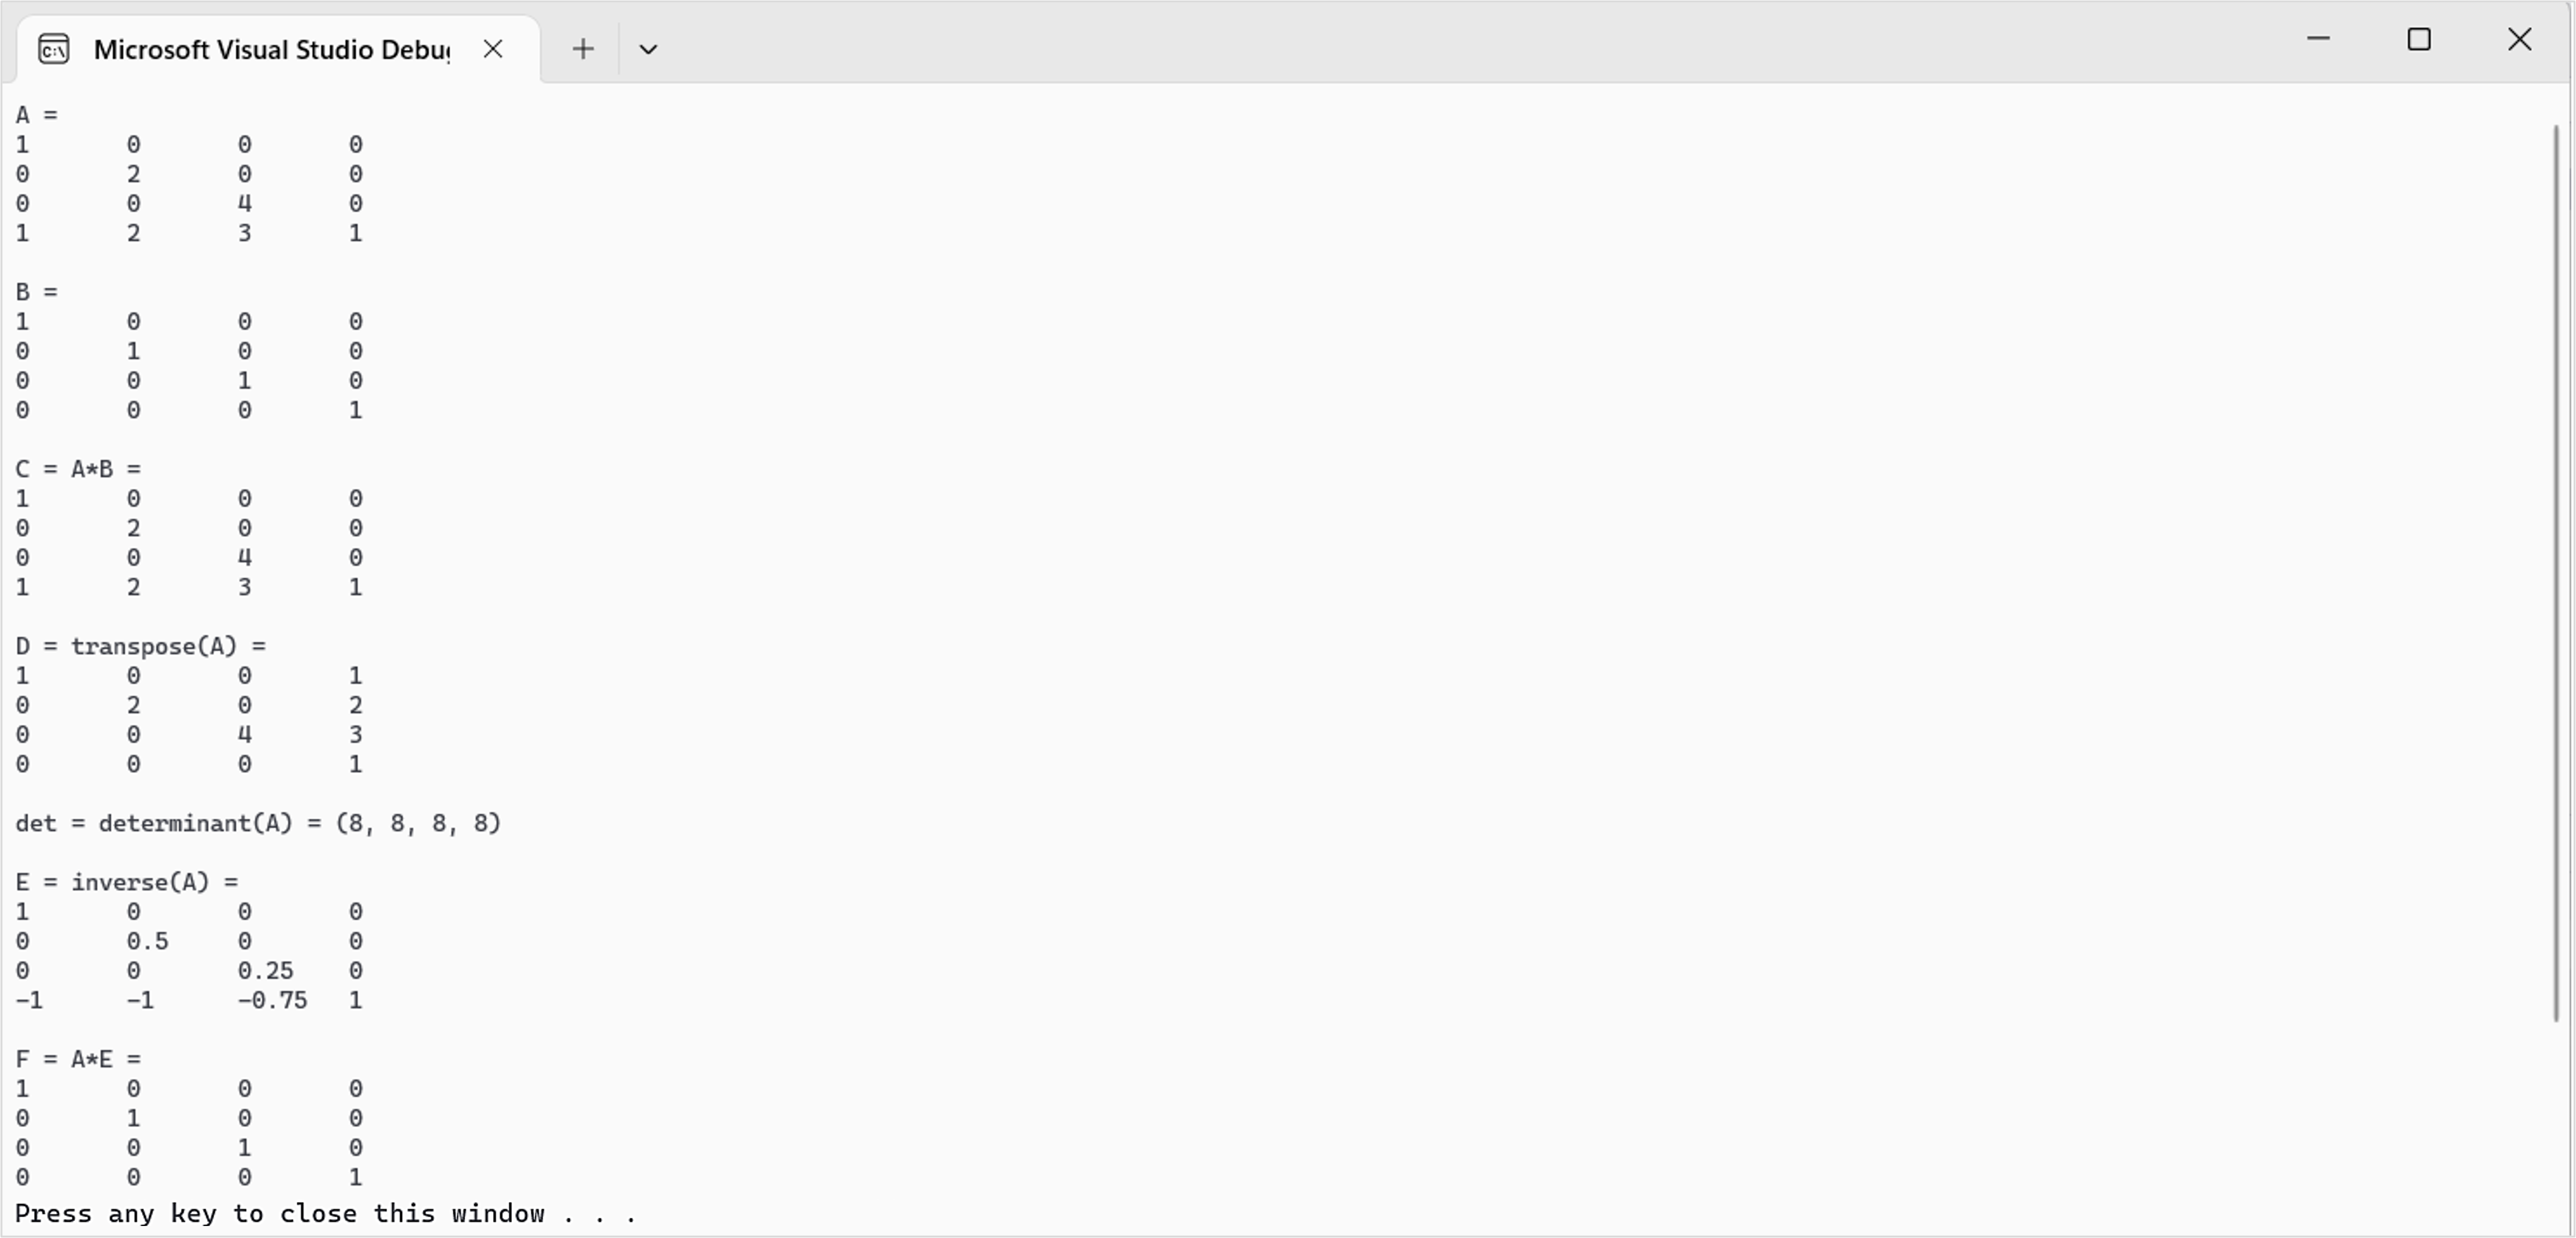
\includegraphics[width=0.8\textwidth]{Images/4/2/4.Session.1.2.1}
            \caption {خروجی برنامه ی بالا.}
            \label{fig:4.Session.1.2.1}
        \end{figure}
    \end{spacing}
}
%-----------------------------------------------------------------------------------------------------------%
\newpage


\section{\textbf{خلاصه}}
\label{sec:2.9}
{
    \Large
    \begin{spacing}{1.5}
        \begin{enumerate}[label=\textbf{\arabic*}.]
            \item {یک ماتریس $m\times n$ $\textbf{A}$ آرایه مستطیلی از اعداد حقیقی با $m$ ردیف و $n$ ستون است.
            دو ماتریس با ابعاد یکسان اگر و تنها اگر اجزای متناظر آنها برابر باشند، مساوی هستند.
            ما دو ماتریس با ابعاد یکسان را با اضافه کردن عناصر متناظر آنها جمع می کنیم.
            ما یک اسکالر و یک ماتریس را با ضرب اسکالر در هر عنصر در ماتریس ضرب می کنیم.}

            \item {اگر $\textbf{A}$ یک ماتریس $m\times n$ و $\textbf{B}$ یک ماتریس $n\times p$ باشد،
            حاصلضرب $\textbf{AB}$ تعریف می شود و یک ماتریس $m\times p$ $\textbf{C}$ است
            که در آن ورودی $ij$مین حاصلضرب $\textbf{C}$ با گرفتن ضرب داخلی بردار ردیف $i$ ام در $\textbf{A}$ با بردار ستون $j$ ام در $\textbf{B}$، یعنی $\textbf{C}^{ij}=\textbf{A}^{i,*}\cdot\textbf{B}^{*,j}$ .}

            \item {ضرب ماتریس جابجایی پذیر نیست (به عنوان مثال، $\textbf{AB}\neq\textbf{BA}$، به طور کلی). ضرب ماتریس شرکت پذیر است: $(\textbf{AB})\textbf{C}=(\textbf{A})\textbf{BC}$.}

            \item {ترانهاده یک ماتریس با تعویض ردیف ها و ستون های ماتریس به دست می آید.
            بنابراین ترانهاده یک ماتریس $m\times n$ یک ماتریس $n\times m$ است.
            ترانهاده یک ماتریس $\textbf{M}$ را $\textbf{M}^{T}$ نشان می دهیم.}

            \item {ماتریس همانی یک ماتریس مربعی است که همه عناصر به جز در امتداد قطر اصلی صفر بوده و عناصر در امتداد قطر اصلی همه یک هستند.}

            \item {دترمینان، \lr{det $\textbf{A}$}، یک تابع ویژه است که یک ماتریس مربعی را دریافت و یک عدد حقیقی را خروجی می دهد.
            یک ماتریس مربعی $\textbf{A}$ معکوس است اگر و تنها اگر $det\textbf{A}\neq 0$ باشد.
            دترمینان در فرمول برای محاسبه معکوس یک ماتریس استفاده می شود.}

            \item {از ضرب یک ماتریس در معکوس آن، ماتریس همانی حاصل می شود: $\textbf{M}\textbf{M}^{-1}=\textbf{M}^{-1}\textbf{M}=\textbf{I}$.
            معکوس یک ماتریس، اگر وجود داشته باشد، منحصر به فرد است.
            فقط ماتریس های مربعی دارای معکوس هستند و حتی در این صورت، ماتریس مربع ممکن است معکوس پذیر نباشد.
            معکوس یک ماتریس را می توان با فرمول محاسبه کرد: $\textbf{A}_{-1}=\textbf{A}^{*}/det\textbf{A}$، که در آن $\textbf{A}^{*}$ الحاق است (ترانهاده ماتریس کوفاکتور $\textbf{A}$).}

            \item {ما از نوع DirectX Math XMMATRIX برای توصیف ماتریس $4\times 4$ به طور موثر در کد با استفاده از عملیات SIMD استفاده می کنیم.
            برای اعضای داده کلاس، ما از کلاس XMFLOAT4X4 استفاده می کنیم و
            سپس از روش های بارگذاری (XMLoadFloat4x4) و ذخیره سازی (XMStoreFloat4x4) برای تبدیل بین XMMATRIX و XMFLOAT4X4 به عقب و جلو استفاده می کنیم.
            کلاس XMMATRIX عملگرهای حسابی را برای انجام جمع، تفریق، ضرب ماتریس و ضرب اسکالر بارگذاری می کند.
            علاوه بر این، کتابخانه ریاضی DirectX توابع ماتریس مفید زیر را برای محاسبه ماتریس همانی، ضرب، ترانهاده، دترمینان و معکوس ارائه می کند:
            \textbf{\vspace{6pt}}
            \lr{\lstinputlisting[language=C++, firstline=198, lastline=203]{Codes/4.1.2.program.c}}
            }
        \end{enumerate}
    \end{spacing}
}
%-----------------------------------------------------------------------------------------------------------%
\newpage


\section{\textbf{تمارین}}
\label{sec:2.10}
{
    \Large
    \begin{spacing}{1.5}
        \begin{enumerate}[label=\textbf{\arabic*}.]
            \item {معادله ماتریسی روبرو را برای $\textbf{X}$ حل کنید: $\left( \begin{bmatrix}
                                                                                  -2 & 0 \\
                                                                                  1  & 3
            \end{bmatrix}-2\textbf{X}=2\begin{bmatrix}
                                           -2 & 0 \\
                                           1  & 3
            \end{bmatrix} \right)$.}

            \item {ضرب های ماتریس زیر را محاسبه کنید: \\
            \lr{
                \begin{flushleft}
                (a)
                    $\begin{bmatrix}
                         -2 & 0 & 3  \\
                         4  & 1 & -1
                    \end{bmatrix}\textbf{X}\begin{bmatrix}
                                               -2 & 1  \\
                                               0  & 6  \\
                                               2  & -3
                    \end{bmatrix}$ \\
                    (b) $\begin{bmatrix}
                             1 & 2 \\
                             3 & 4
                    \end{bmatrix}\textbf{X}\begin{bmatrix}
                                               -2 & 0 \\
                                               1  & 1
                    \end{bmatrix}$ \\
                    (c) $\begin{bmatrix}
                             2 & 0  & 2  \\
                             0 & -1 & -3 \\
                             0 & 0  & 1
                    \end{bmatrix}\textbf{X}\begin{bmatrix}
                                               1 \\
                                               2 \\
                                               1
                    \end{bmatrix}$
                \end{flushleft}
            }
            }

            \item {ترانهاده ماتریس های زیر را محاسبه کنید: \\
            \lr{
                \begin{flushleft}
                (a)
                    $[1, 2, 3]$ \\
                    (b) $\begin{bmatrix}
                             x & y \\
                             z & w
                    \end{bmatrix}$ \\
                    (c) $\begin{bmatrix}
                             1 & 2 \\
                             3 & 4 \\
                             5 & 6 \\
                             7 & 8
                    \end{bmatrix}$
                \end{flushleft}
            }
            }

            \item {نشان دهید: \\
                \begin{center}
                    $\textbf{AB}=\begin{bmatrix}
                                     A_{11} & A_{12} & A_{13} \\
                                     A_{21} & A_{22} & A_{23} \\
                                     A_{31} & A_{32} & A_{33}
                    \end{bmatrix}\begin{bmatrix}
                                     B_{11} & B_{12} \\
                                     B_{21} & B_{22} \\
                                     B_{31} & B_{32}
                    \end{bmatrix}=\begin{bmatrix}
                                      \leftarrow & \textbf{A}_{1,*}\textbf{B} & \rightarrow \\
                                      \leftarrow & \textbf{A}_{2,*}\textbf{B} & \rightarrow \\
                                      \leftarrow & \textbf{A}_{3,*}\textbf{B} & \rightarrow
                    \end{bmatrix}$
                \end{center}
            }

            \item {نشان دهید: \\
                \begin{center}
                    $\textbf{Au}=\begin{bmatrix}
                                     A_{11} & A_{12} & A_{13} \\
                                     A_{21} & A_{22} & A_{23} \\
                                     A_{31} & A_{32} & A_{33}
                    \end{bmatrix}\begin{bmatrix}
                                     x \\
                                     y \\
                                     z
                    \end{bmatrix}=x\textbf{A}_{*,1}+y\textbf{A}_{*,2}+z\textbf{A}_{*,3}$
                \end{center}
            }

            \item {ثابت کنید که ضرب خارجی را می توان با ضرب ماتریس بیان کرد:
                \begin{center}
                    $\textbf{u}\times\textbf{v}=\begin{bmatrix}
                                                    v_{x} & v_{y} & v_{z}
                    \end{bmatrix}\begin{bmatrix}
                                     0      & u_{z}  & -u_{y} \\
                                     -u_{z} & 0      & u_{x}  \\
                                     u_{y}  & -u_{x} & 0
                    \end{bmatrix}$
                \end{center}
            }

            \item {فرض کنید $\textbf{A}=\begin{bmatrix}
                                            2 & 0  & 1  \\
                                            0 & -1 & -3 \\
                                            0 & 0  & 1
            \end{bmatrix}$. آیا $\textbf{B}=\begin{bmatrix}
                                                1/2 & 0  & -1/2 \\
                                                0   & -1 & -3   \\
                                                0   & 0  & 1
            \end{bmatrix}$ ترانهاده ی $\textbf{A}$ است؟
            }

            \item {فرض کنید $\textbf{A}=\begin{bmatrix}
                                            1 & 2 \\
                                            3 & 4
            \end{bmatrix}$. آیا $\textbf{B}=\begin{bmatrix}
                                                -2  & 1   \\
                                                3/2 & 1/2
            \end{bmatrix}$ ترانهاده ی $\textbf{A}$ است؟
            }

            \item {دترمینان های ماتریس های زیر را بیابید:
                $\begin{bmatrix}
                     21 & -4 \\
                     10 & 7
                \end{bmatrix}$,
                $\begin{bmatrix}
                     2 & 0 & 0 \\
                     0 & 3 & 0 \\
                     0 & 0 & 7
                \end{bmatrix}$
            }

            \item {معکوس ماتریس های زیر را بیابید:
                $\begin{bmatrix}
                     21 & -4 \\
                     10 & 7
                \end{bmatrix}$,
                $\begin{bmatrix}
                     2 & 0 & 0 \\
                     0 & 3 & 0 \\
                     0 & 0 & 7
                \end{bmatrix}$
            }

            \item {آیا ماتریس زیر معکوس پذیر است؟
                \begin{center}
                    $\begin{bmatrix}
                         1 & 2 & 3 \\
                         0 & 4 & 5 \\
                         0 & 0 & 0
                    \end{bmatrix}$
                \end{center}
            }

            \item {نشان دهید که $(\textbf{A}^{-1})^{T}=(\textbf{A}^{T})^{-1}$، با فرض اینکه $\textbf{A}$ معکوس پذیر است.}

            \item {فرض کنید $\textbf{A}$ و $\textbf{B}$ ماتریس $n\times n$ باشند.
            ک واقعیت ثابت شده در کتاب های جبر خطی این است که $det\textbf{AB}=det\textbf{A}\cdot\textbf{B}$.
            از این واقعیت به همراه این واقعیت که $det\textbf{I}=1$ برای اثبات $\textbf{A}^{-1}=\frac{\displaystyle 1}{\displaystyle det\textbf{A}}$ استفاده کنید،
            با فرض اینکه $\textbf{A}$ معکوس پذیر است.}

            \item {ثابت کنید که دترمینان دوبعدی  $\begin{bmatrix}
                                                      u_{x} & u_{y} \\
                                                      v_{x} & v_{y}
            \end{bmatrix}$ مساحت علامت متوازی الاضلاع را می دهد که با $\textbf{u}=(u_{x},u_{y})$ و $\textbf{v}=(v_{x},v_{y})$ پوشیده شده است.
            نتیجه مثبت است اگر $\textbf{u}$ را بتوان در خلاف جهت عقربه های ساعت بچرخانیم تا با $\textbf{v}$ با زاویه $\theta\in(0,\pi)$ منطبق شود، و در غیر این صورت منفی است.
                \begin{figure}[H]
                    \centering
                    \setlength{\belowcaptionskip}{-10pt}
                    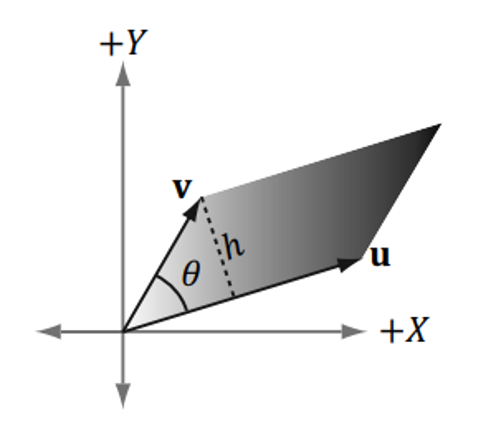
\includegraphics[width=0.5\textwidth]{Images/4/2/4.Session.1.2.2}
                    \label{fig:4.Session.1.2.2}
                \end{figure}
            }

            \item {مساحت متوازی الاضلاع را بیابید که با موارد زیر پوشیده شده باشد: \\
            \lr{(a) $\textbf{u}=(3,0), \textbf{v}=(1,1)$}
            \lr{(b) $\textbf{u}=(-1,-1), \textbf{v}=(0,1)$}
            }

            \item {فرض کنید $\textbf{A}=\begin{bmatrix}
                                            A_{11} & A_{12} \\
                                            A_{21} & A_{22}
            \end{bmatrix}$، $\textbf{B}=\begin{bmatrix}
                                            B_{11} & B_{12} \\
                                            B_{21} & B_{22}
            \end{bmatrix}$ و $\textbf{C}=\begin{bmatrix}
                                             C_{11} & C_{12} \\
                                             C_{21} & C_{22}
            \end{bmatrix}$ نشان دهید که $\textbf{A}(\textbf{BC})=(\textbf{AB})\textbf{C}$.
            این نشان می دهد که ضرب ماتریس برای ماتریس های $2\times 2$ شرکت پذیر است.
                (در واقع، هر زمان که ضرب تعریف شود، ضرب ماتریس برای ماتریس‌های با اندازه عمومی شرکت پذیر است.)}

            \item {یک برنامه کامپیوتری بنویسید که ترانهاده یک ماتریس $m\times n$ را بدون استفاده از \lr{DirectX Math} محاسبه کند
                (فقط از آرایه ای از آرایه ها در \lr{C++} استفاده کنید).}

            \item {یک برنامه کامپیوتری بنویسید که دترمینان و معکوس ماتریس های $4\times 4$ را بدون استفاده از \lr{DirectX Math} محاسبه کند
                (فقط از آرایه ای از آرایه ها در \lr{C++} استفاده کنید).}
        \end{enumerate}
    \end{spacing}
}